\documentclass[a4paper,12pt]{article}

\usepackage[english]{babel}
\usepackage{graphicx}
\usepackage{amsmath}
\usepackage{hyperref}
\hypersetup{
    colorlinks=false,
    pdfborder={0 0 0},
}


\title{Some simple algorithms for detecting anomalous bright pixels}
\author{Alessandro Gentilini\thanks{alessandro.gentilini@gmail.com}}


\begin{document}
\maketitle

\begin{abstract}
I describe some simple algorithms I am using for detecting anomalous bright 
pixels in images taken by a laptop webcam.
The webcam lens is covered with black tape and so the visible light is not 
collected by the sensor; the grey levels different from zero in the image are 
usually due to the so called \emph{dark current}; sometimes there are bright 
pixels (and I classify the image as an \emph{event}) and an hypothesis is that 
the bright pixels are the result of the interaction of cosmic ray muons with the 
semiconductor sensor of the webcam.
\end{abstract} 

\section{Algorithms}
I am experimenting various algorithms in order to classify an image as an 
\emph{event}.

I have a sequence of images, let $I_i$ be the $i$-th image in the sequence. The 
image has $R$ rows and $C$ columns. Let $I_i(r,c)$ be the grey value of the pixel 
at $row=r$ and $column=c$ in the image $I_i$.
The program computes $M_i$ as 
$$M_i=\max_{\substack{
   0\leq r\leq R-1 \\
   0\leq c\leq C-1
  }}
 I_i(r,c)$$

So $M_i$ is the maximum grey level in the image $I_i$.\\

The simplest algorithm uses a fixed threshold $t$ and the image $I_i$ is 
classified as an event if 
\begin{equation}
M_i>t \label{eq:1}
\end{equation}

For example formula \ref{eq:1} is used in 
\texttt{dkirkby/cosmic}\footnote{\emph{Cosmic ray detector for iOS} available at 
\url{https://github.com/dkirkby/cosmic}} with an additional filter stage with 
the aim to filter out the so-called \emph{hot pixels}. If the maximum grey level 
$M_i$ happens at the same pixel position $(r_H,c_H)$ more than a certain number 
of times then the pixel at $(r_H,c_H)$ is classified as an hot pixel and any 
following images with maximum at $(r_H,c_H)$ is discarded\footnote{See 
\url{https://github.com/dkirkby/cosmic/blob/master/Cosmic/CosmicBrain.m} 
accessed March 2, 2014, where the number of time is \texttt{MAX\_REPEATS} 
and the threshold $t$ is \texttt{MIN\_INTENSITY}.}.\\

A different algorithm considers the average grey level $avg_i$ of the image 
$I_i$ and the standard deviation $sd_i$ of the grey levels of the image $I_i$, 
the image $I_i$ is then classified as an event if 

\begin{equation}
M_i>avg_i+n\cdot sd_i
\end{equation}\\

In a third algorithm, the program keeps running statistics for $M_i$, in 
particular $\overline{M}_i$ is the mean of the maximum grey levels and it is 
computed as

$$\overline{M}_i=\frac{1}{i}\sum_{k=1}^i M_k$$

and ${\sigma_{M}}_{i}$ is the standard deviation of the maximum grey level and 
it is computed as

$${\sigma_{M}}_{i}=\sqrt{\frac{1}{i(i-1)}\left(i\sum_{k=1}^i {M_k}^2-\left(\sum_{k=1}^i M_k\right)^2\right)}$$


The image $I_i$ is then considered an event if 
\begin{equation}
M_i>\overline{M}_i+n\cdot{\sigma_{M}}_{i}\label{eq:3}
\end{equation}

\begin{figure}[h!]
  \centering
  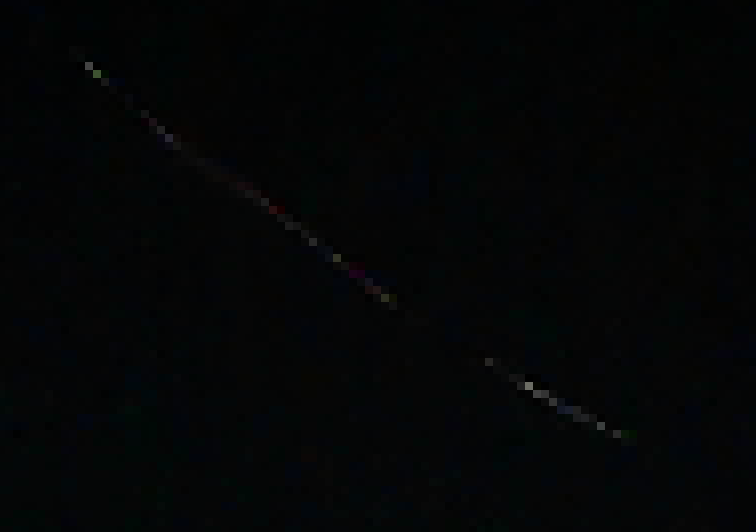
\includegraphics[scale=0.5]{bella.png}
  \caption{A crop from an image classified as an event using formula \ref{eq:3} 
  with $n=10$.}
\end{figure}

\section{Data}
Figures \ref{fig:1} to \ref{fig:2} show data collected in various days.
The time between two images acquisition has a mean value of 0.13s and a standard 
deviation of 8ms.
The exposure time is unknown.
The images were collected with a laptop webcam, the location is in Northern 
Italy, the time is local.

The graphs should be considered as a work in progress, in particular I have some 
issues with them:
\begin{enumerate}
  \item The range for $M_i$ in Figures \ref{fig:1} and \ref{fig:3} seems quite 
  different with respect to the remaining Figures.
  \item The curve for $\overline{M}_i$ seems too low in Figure \ref{fig:1} 
  and \ref{fig:3}.
  \item The curve for $\overline{M}_i$ does not properly follow the trend of 
  $M_i$ in Figures 
  \ref{fig:4} and \ref{fig:2}.
\end{enumerate}
The above issues could have been caused by some errors in the program collecting 
the data, I should investigate further.\\

The summary for the hourly rate event is the following:
\begin{verbatim}
   Min. 1st Qu.  Median    Mean 3rd Qu.    Max. 
  0.700   1.355   1.840   1.991   2.468   4.460
\end{verbatim}

This table summarize the data collected so far.
% latex table generated in R 3.0.2 by xtable 1.7-1 package
% Wed Feb 26 20:08:57 2014
\begin{table}[ht]
\centering
\begin{tabular}{rrr}
  \hline
 events & elapsed time & events per hour \\ 
  \hline
   9 & 03h14m18s & 2.78 \\ 
   12 & 08h03m03s & 1.49 \\ 
   23 & 09h27m57s & 2.43 \\ 
   15 & 06h37m57s & 2.26 \\ 
    6 & 08h37m23s & 0.70 \\ 
   10 & 08h06m30s & 1.23 \\ 
    8 & 09h05m33s & 0.88 \\ 
   22 & 08h44m34s & 2.52 \\ 
   17 & 08h44m33s & 1.94 \\ 
    7 & 05h21m33s & 1.31 \\ 
   12 & 07h16m38s & 1.65 \\ 
   11 & 06h19m07s & 1.74 \\ 
   20 & 08h04m50s & 2.48 \\ 
   \hline
\end{tabular}
\end{table}


\begin{figure}[h!]
  \centering
  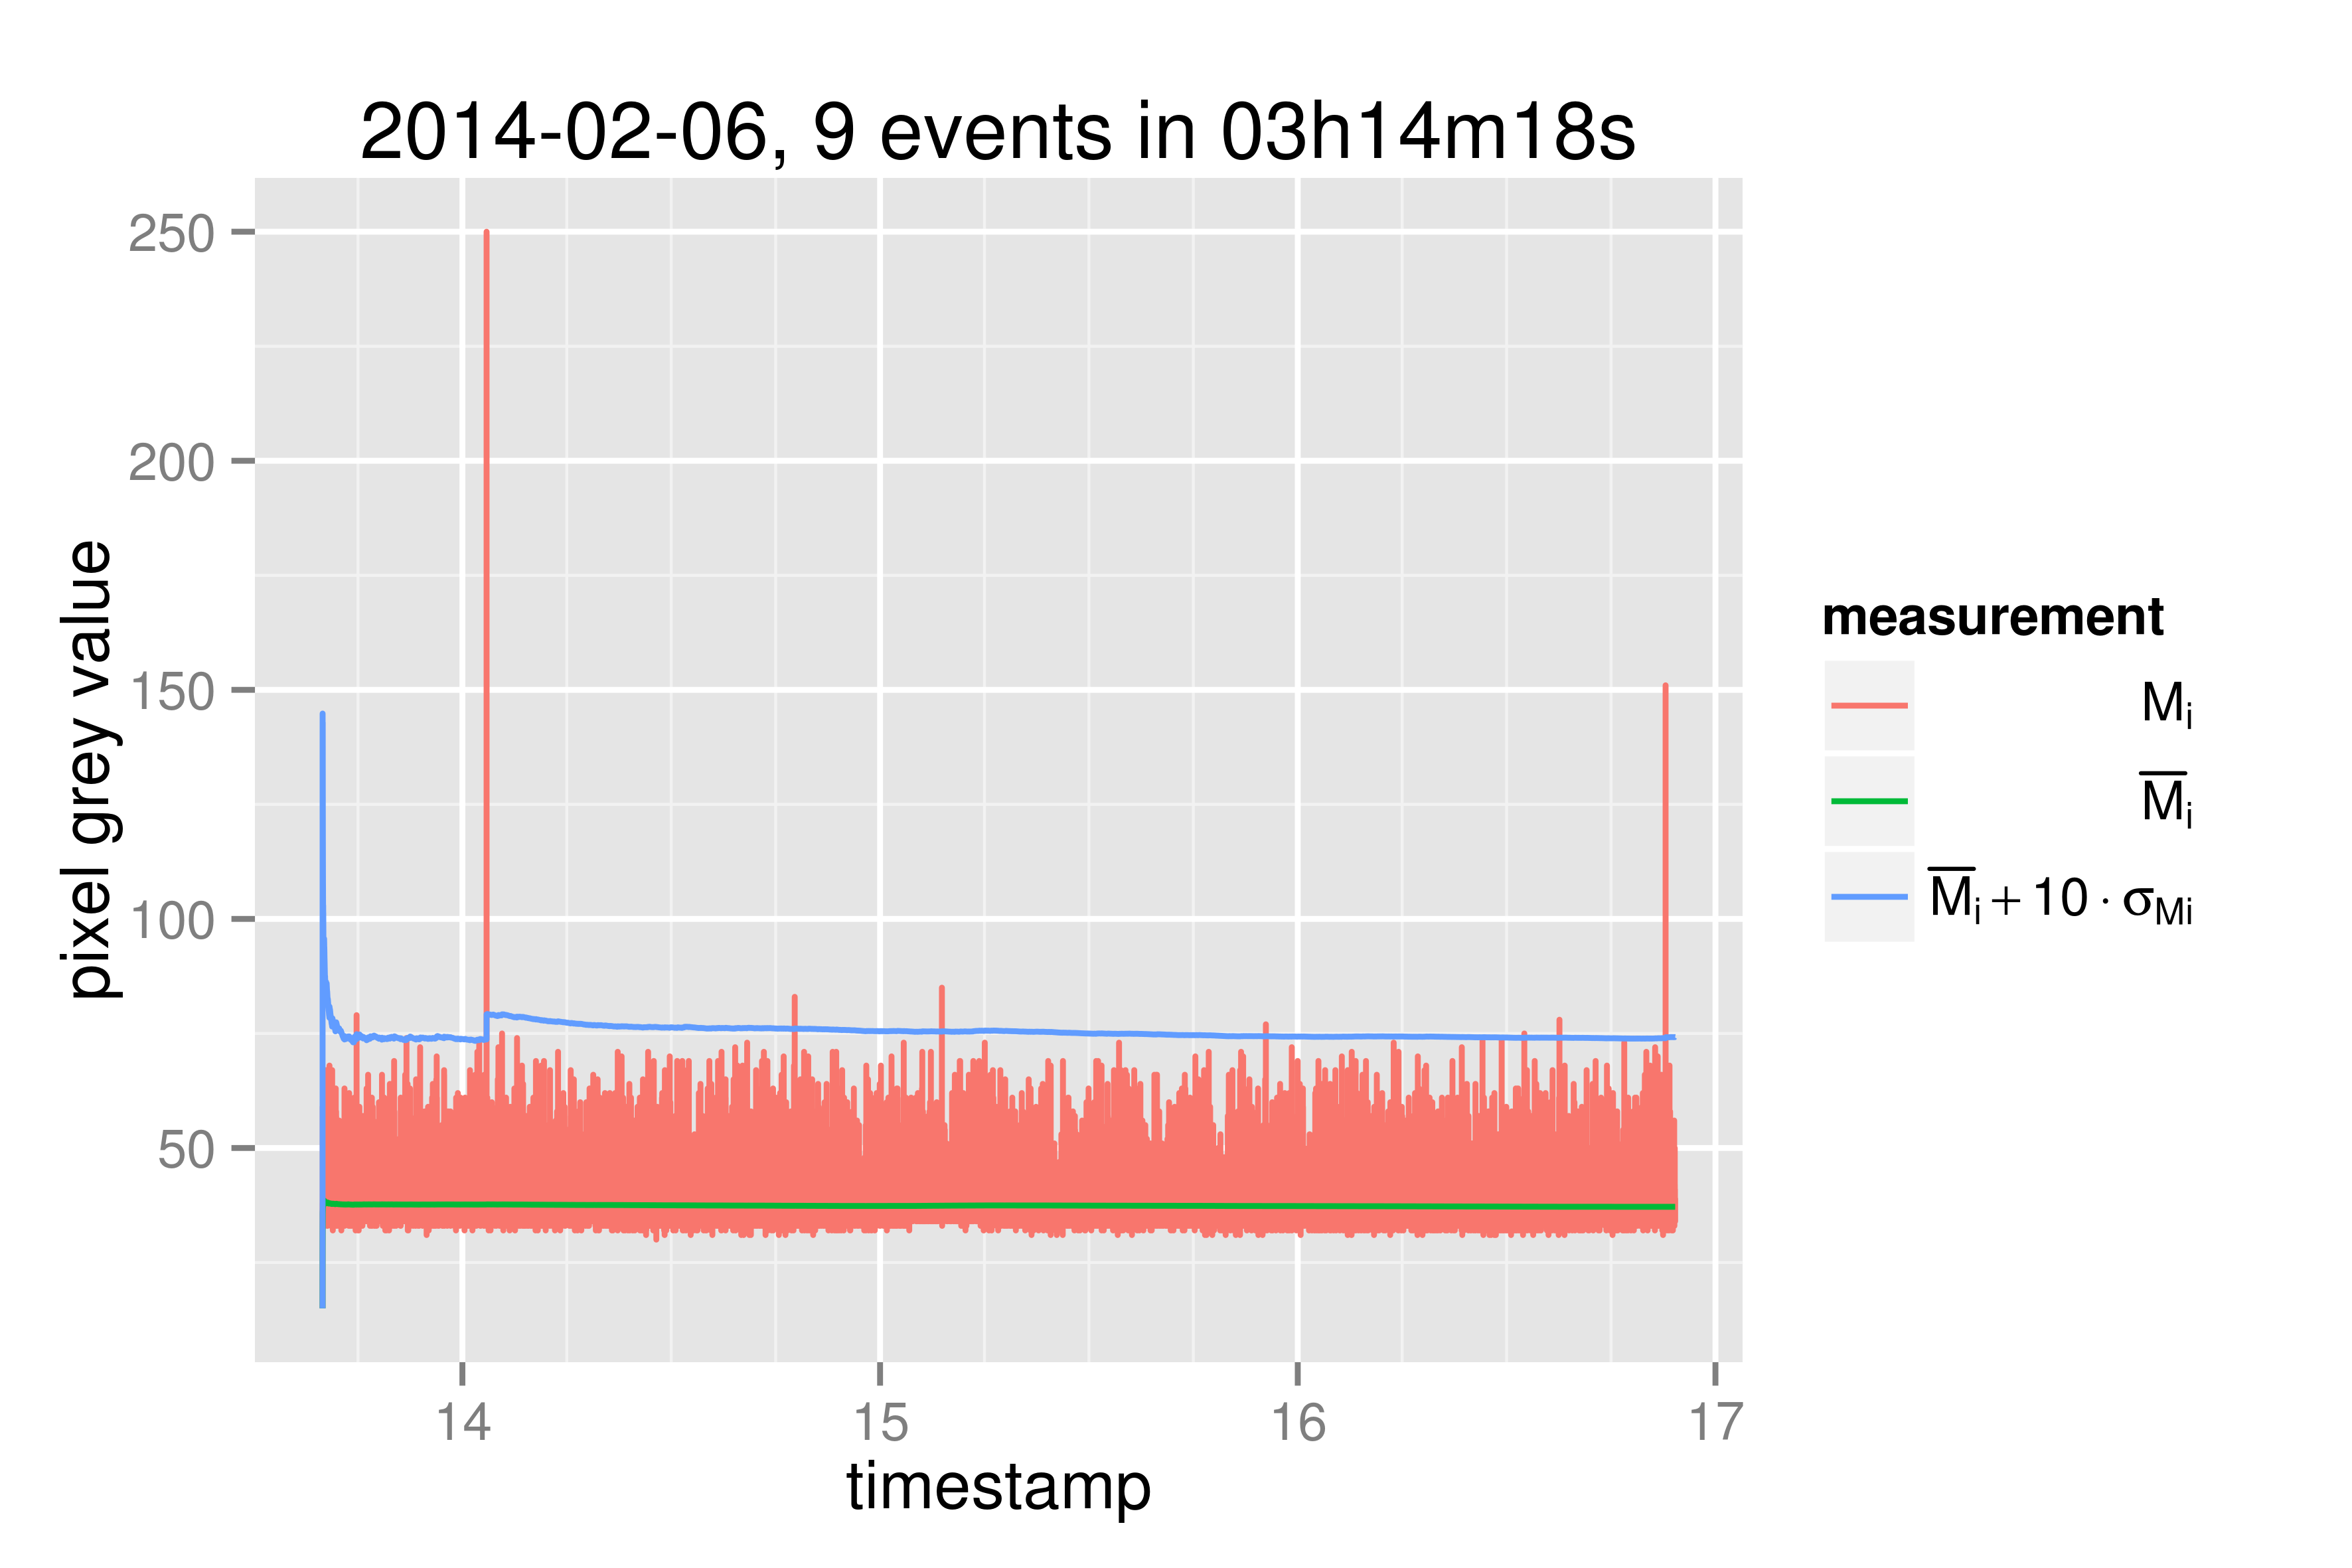
\includegraphics{20140206.png}
  \caption{Data collected using formula \ref{eq:3} with $n=10$.}\label{fig:1}
\end{figure}

\begin{figure}[h!]
  \centering
  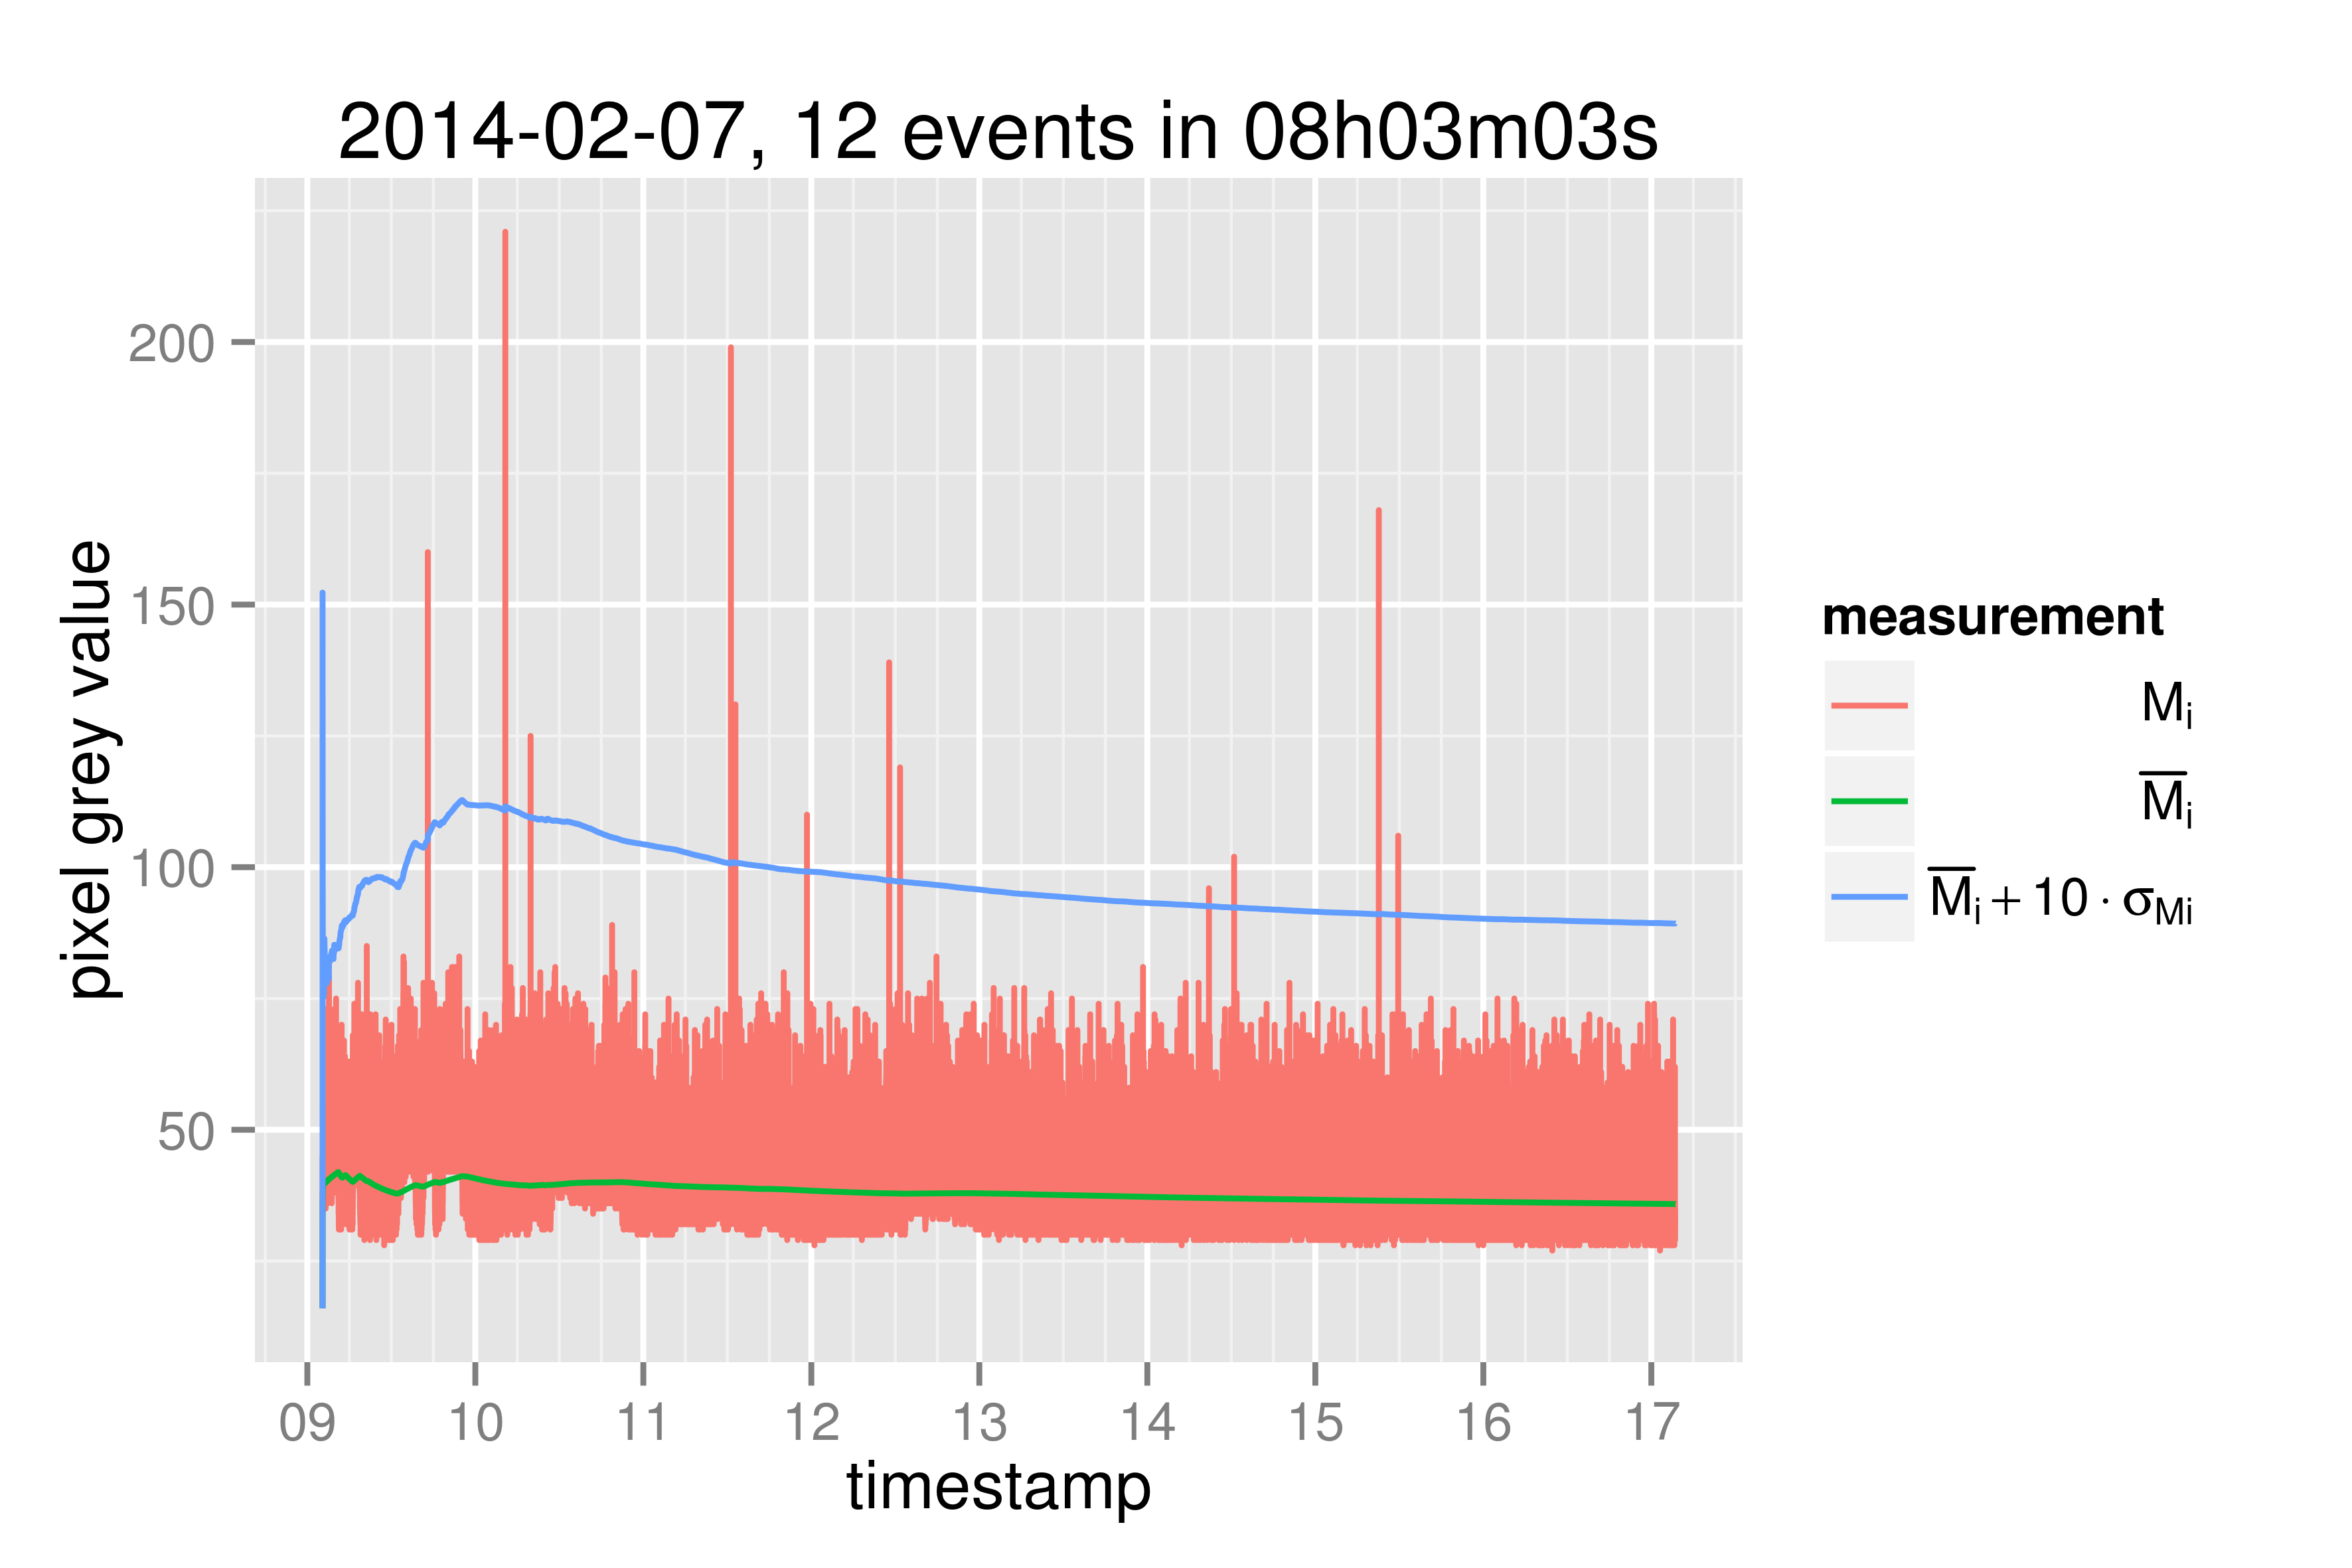
\includegraphics{20140207.png}
  \caption{Data collected using formula \ref{eq:3} with $n=10$.}\label{fig:3}
\end{figure}

\begin{figure}[h!]
  \centering
  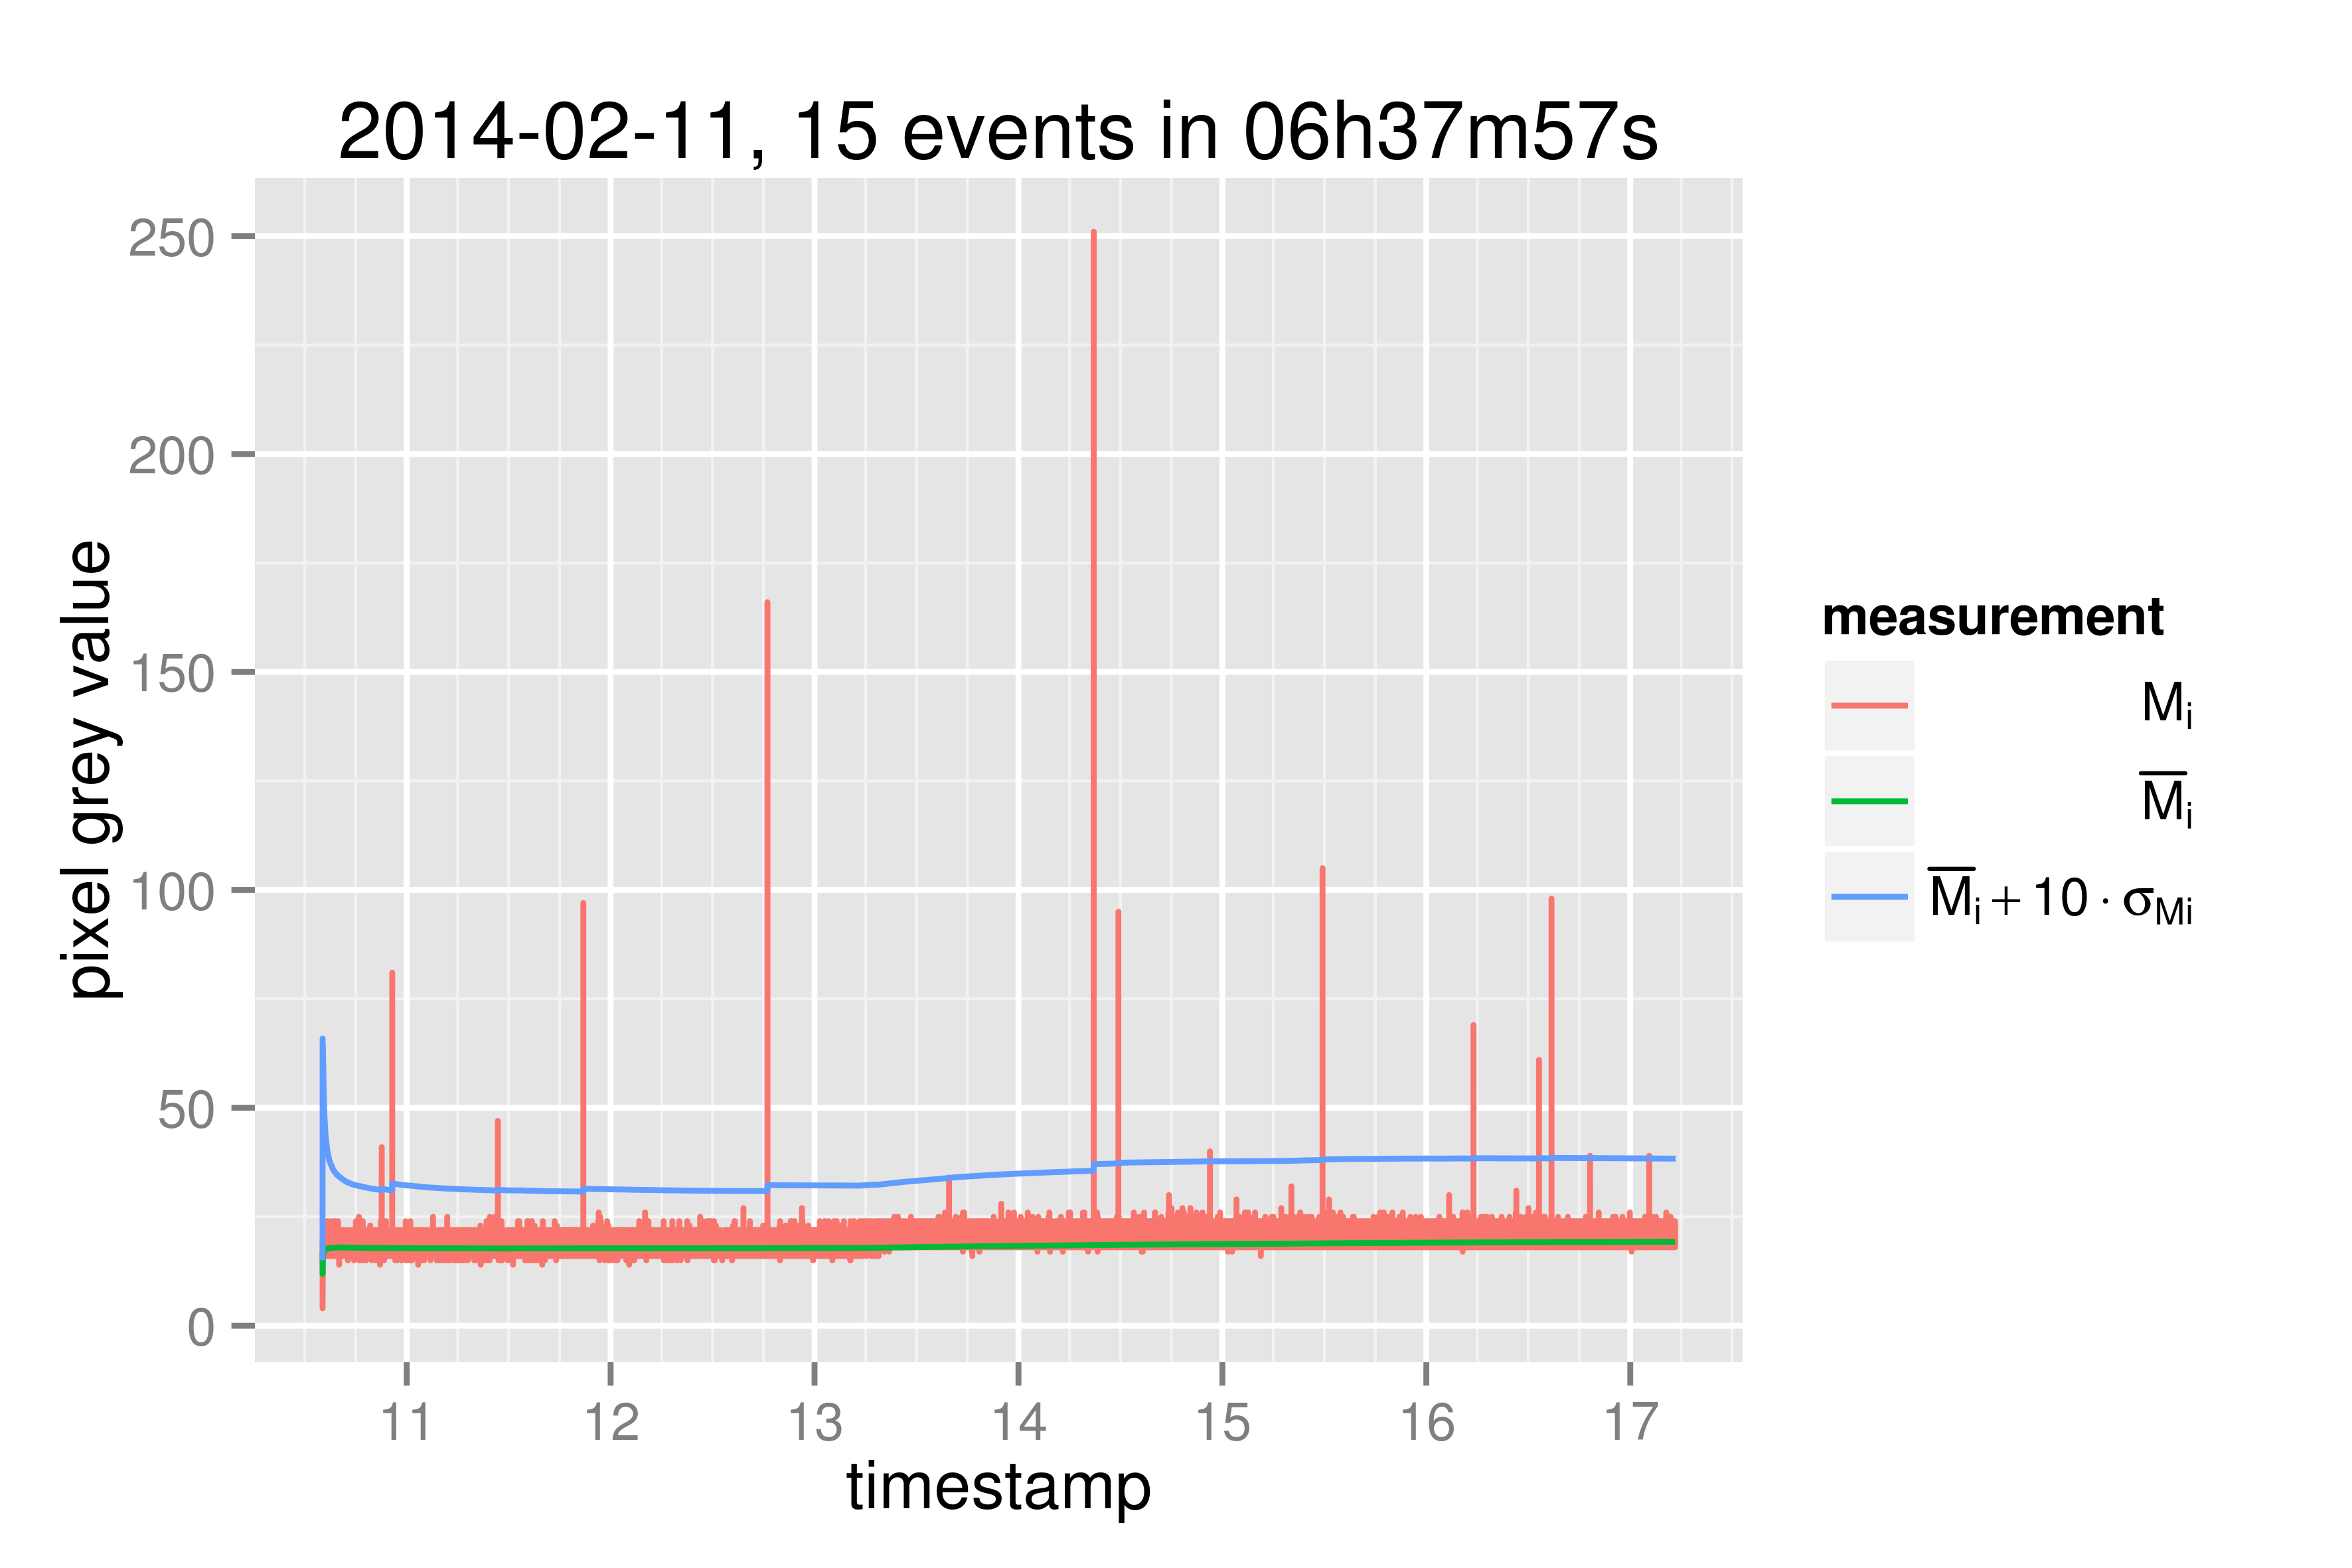
\includegraphics{20140211.png}
  \caption{Data collected using formula \ref{eq:3} with $n=10$.}
\end{figure}

\begin{figure}[h!]
  \centering
  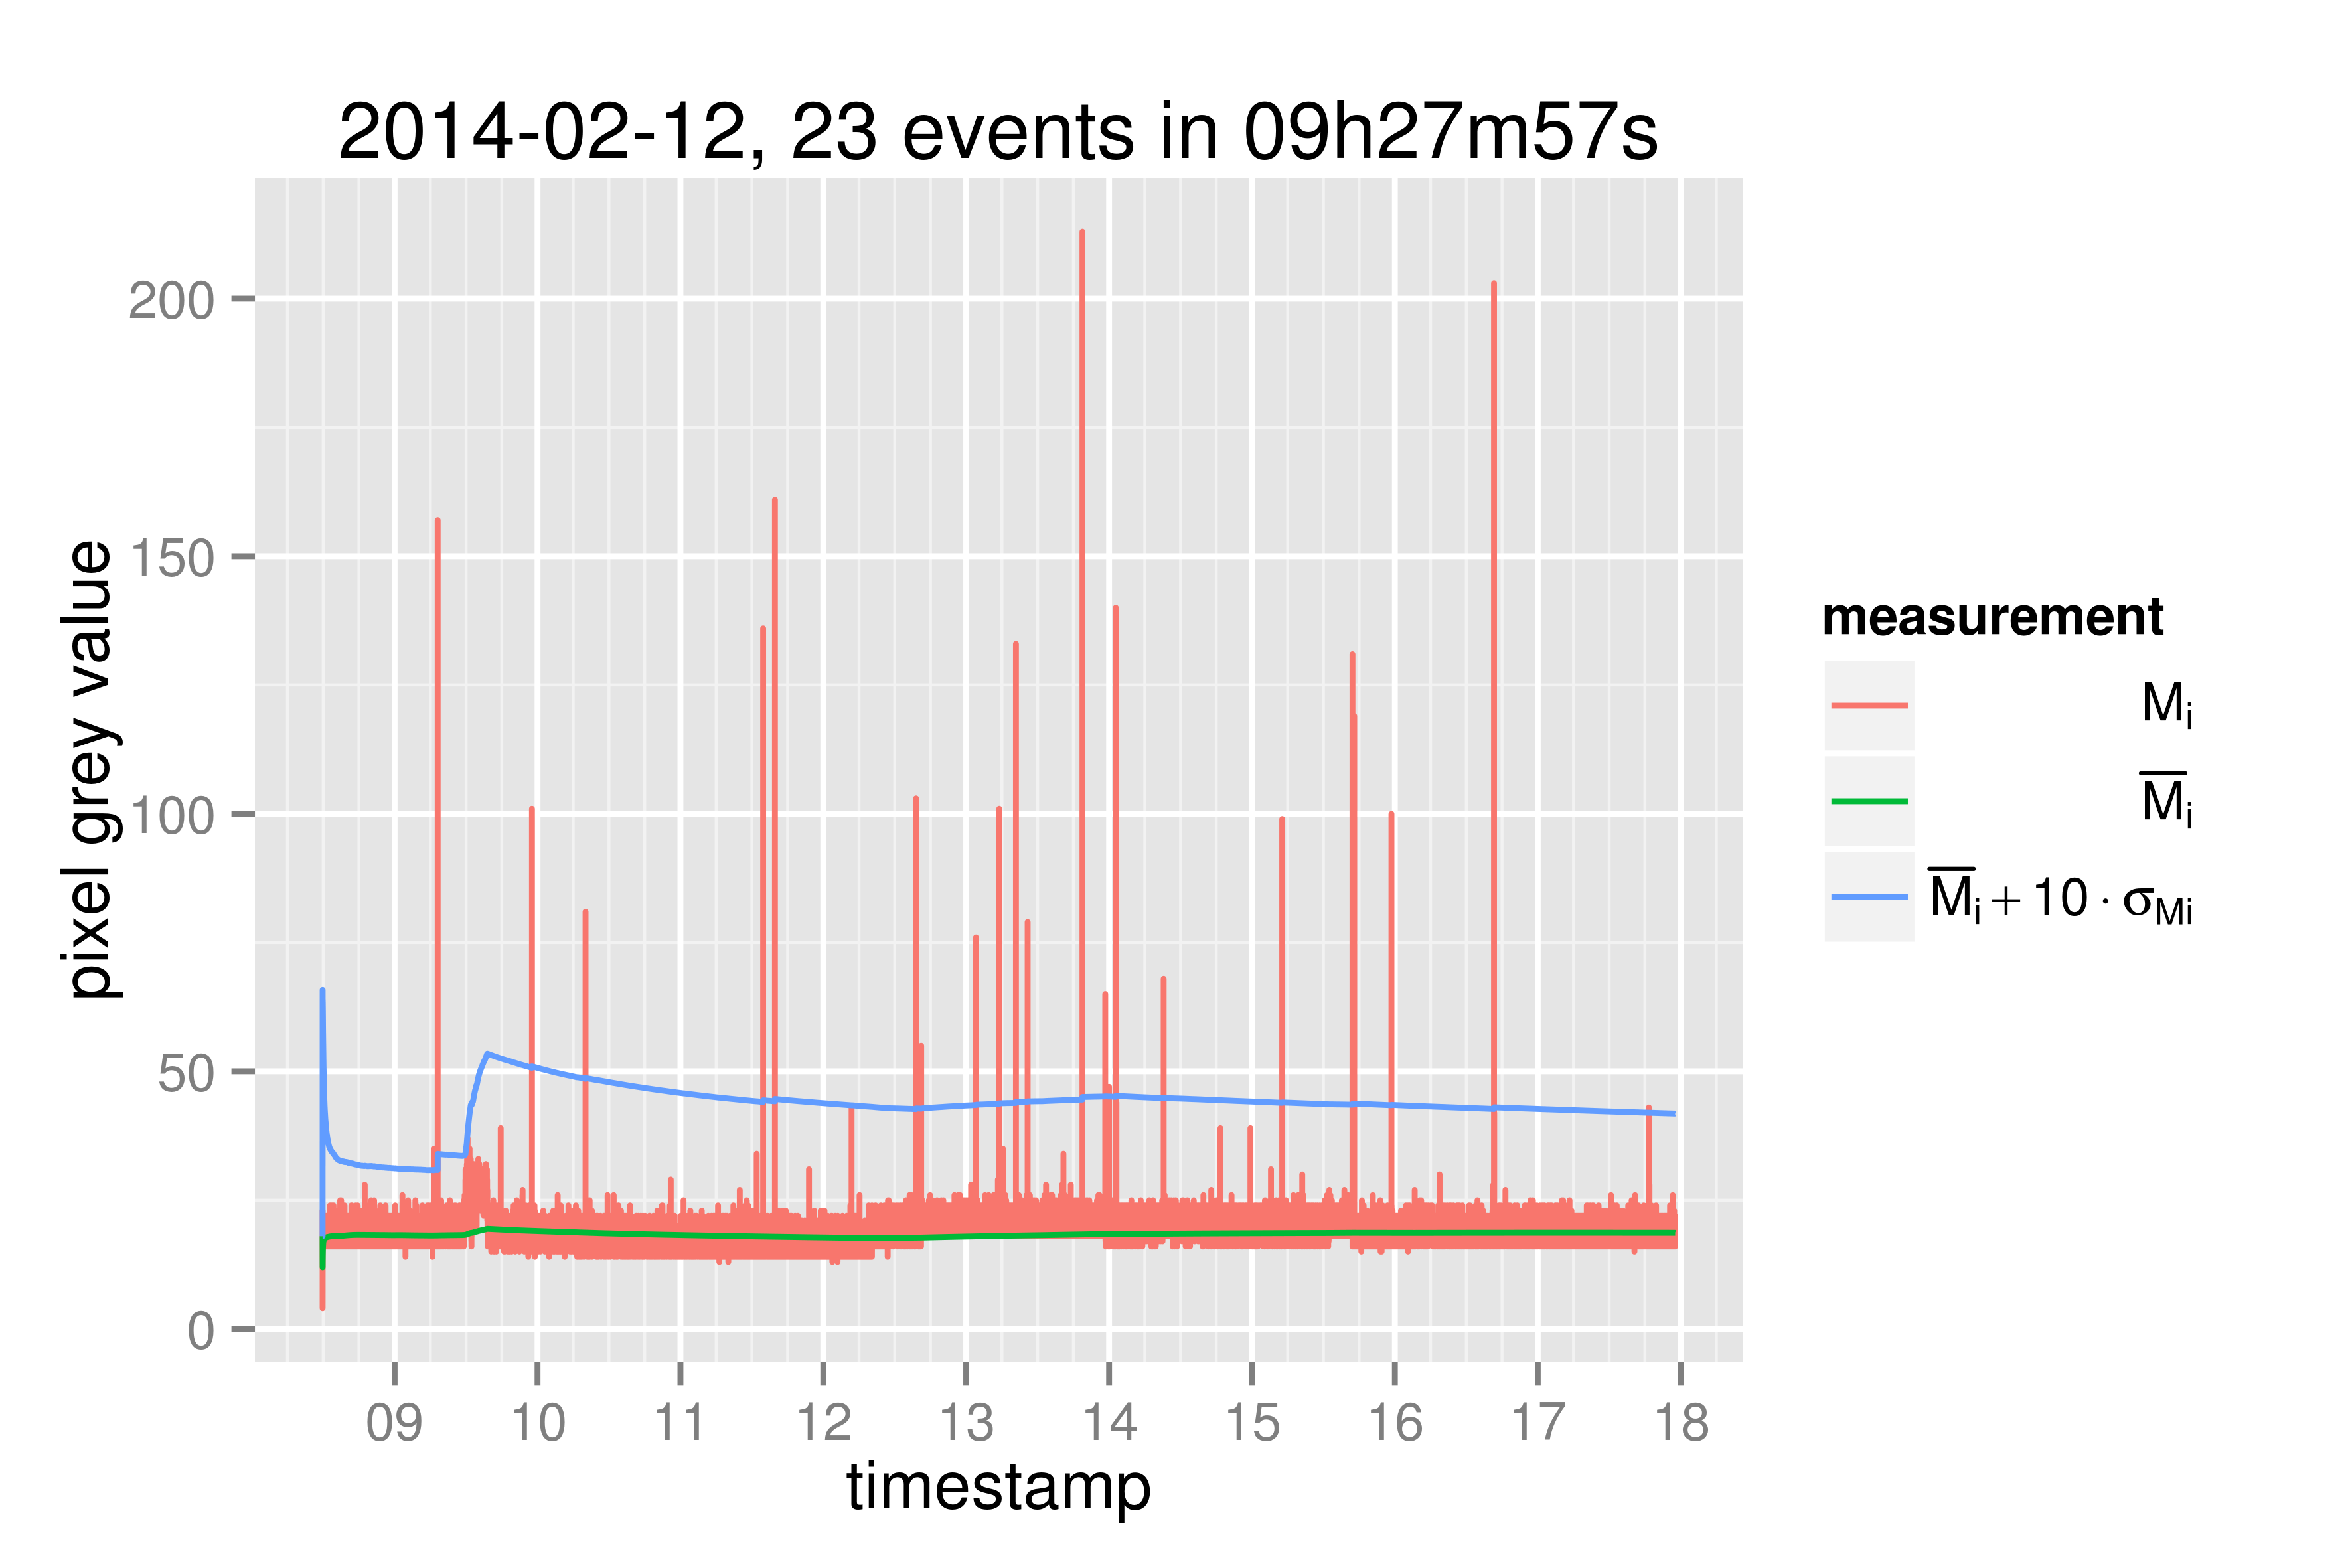
\includegraphics{20140212.png}
  \caption{Data collected using formula \ref{eq:3} with $n=10$.}
\end{figure}

\begin{figure}[h!]
  \centering
  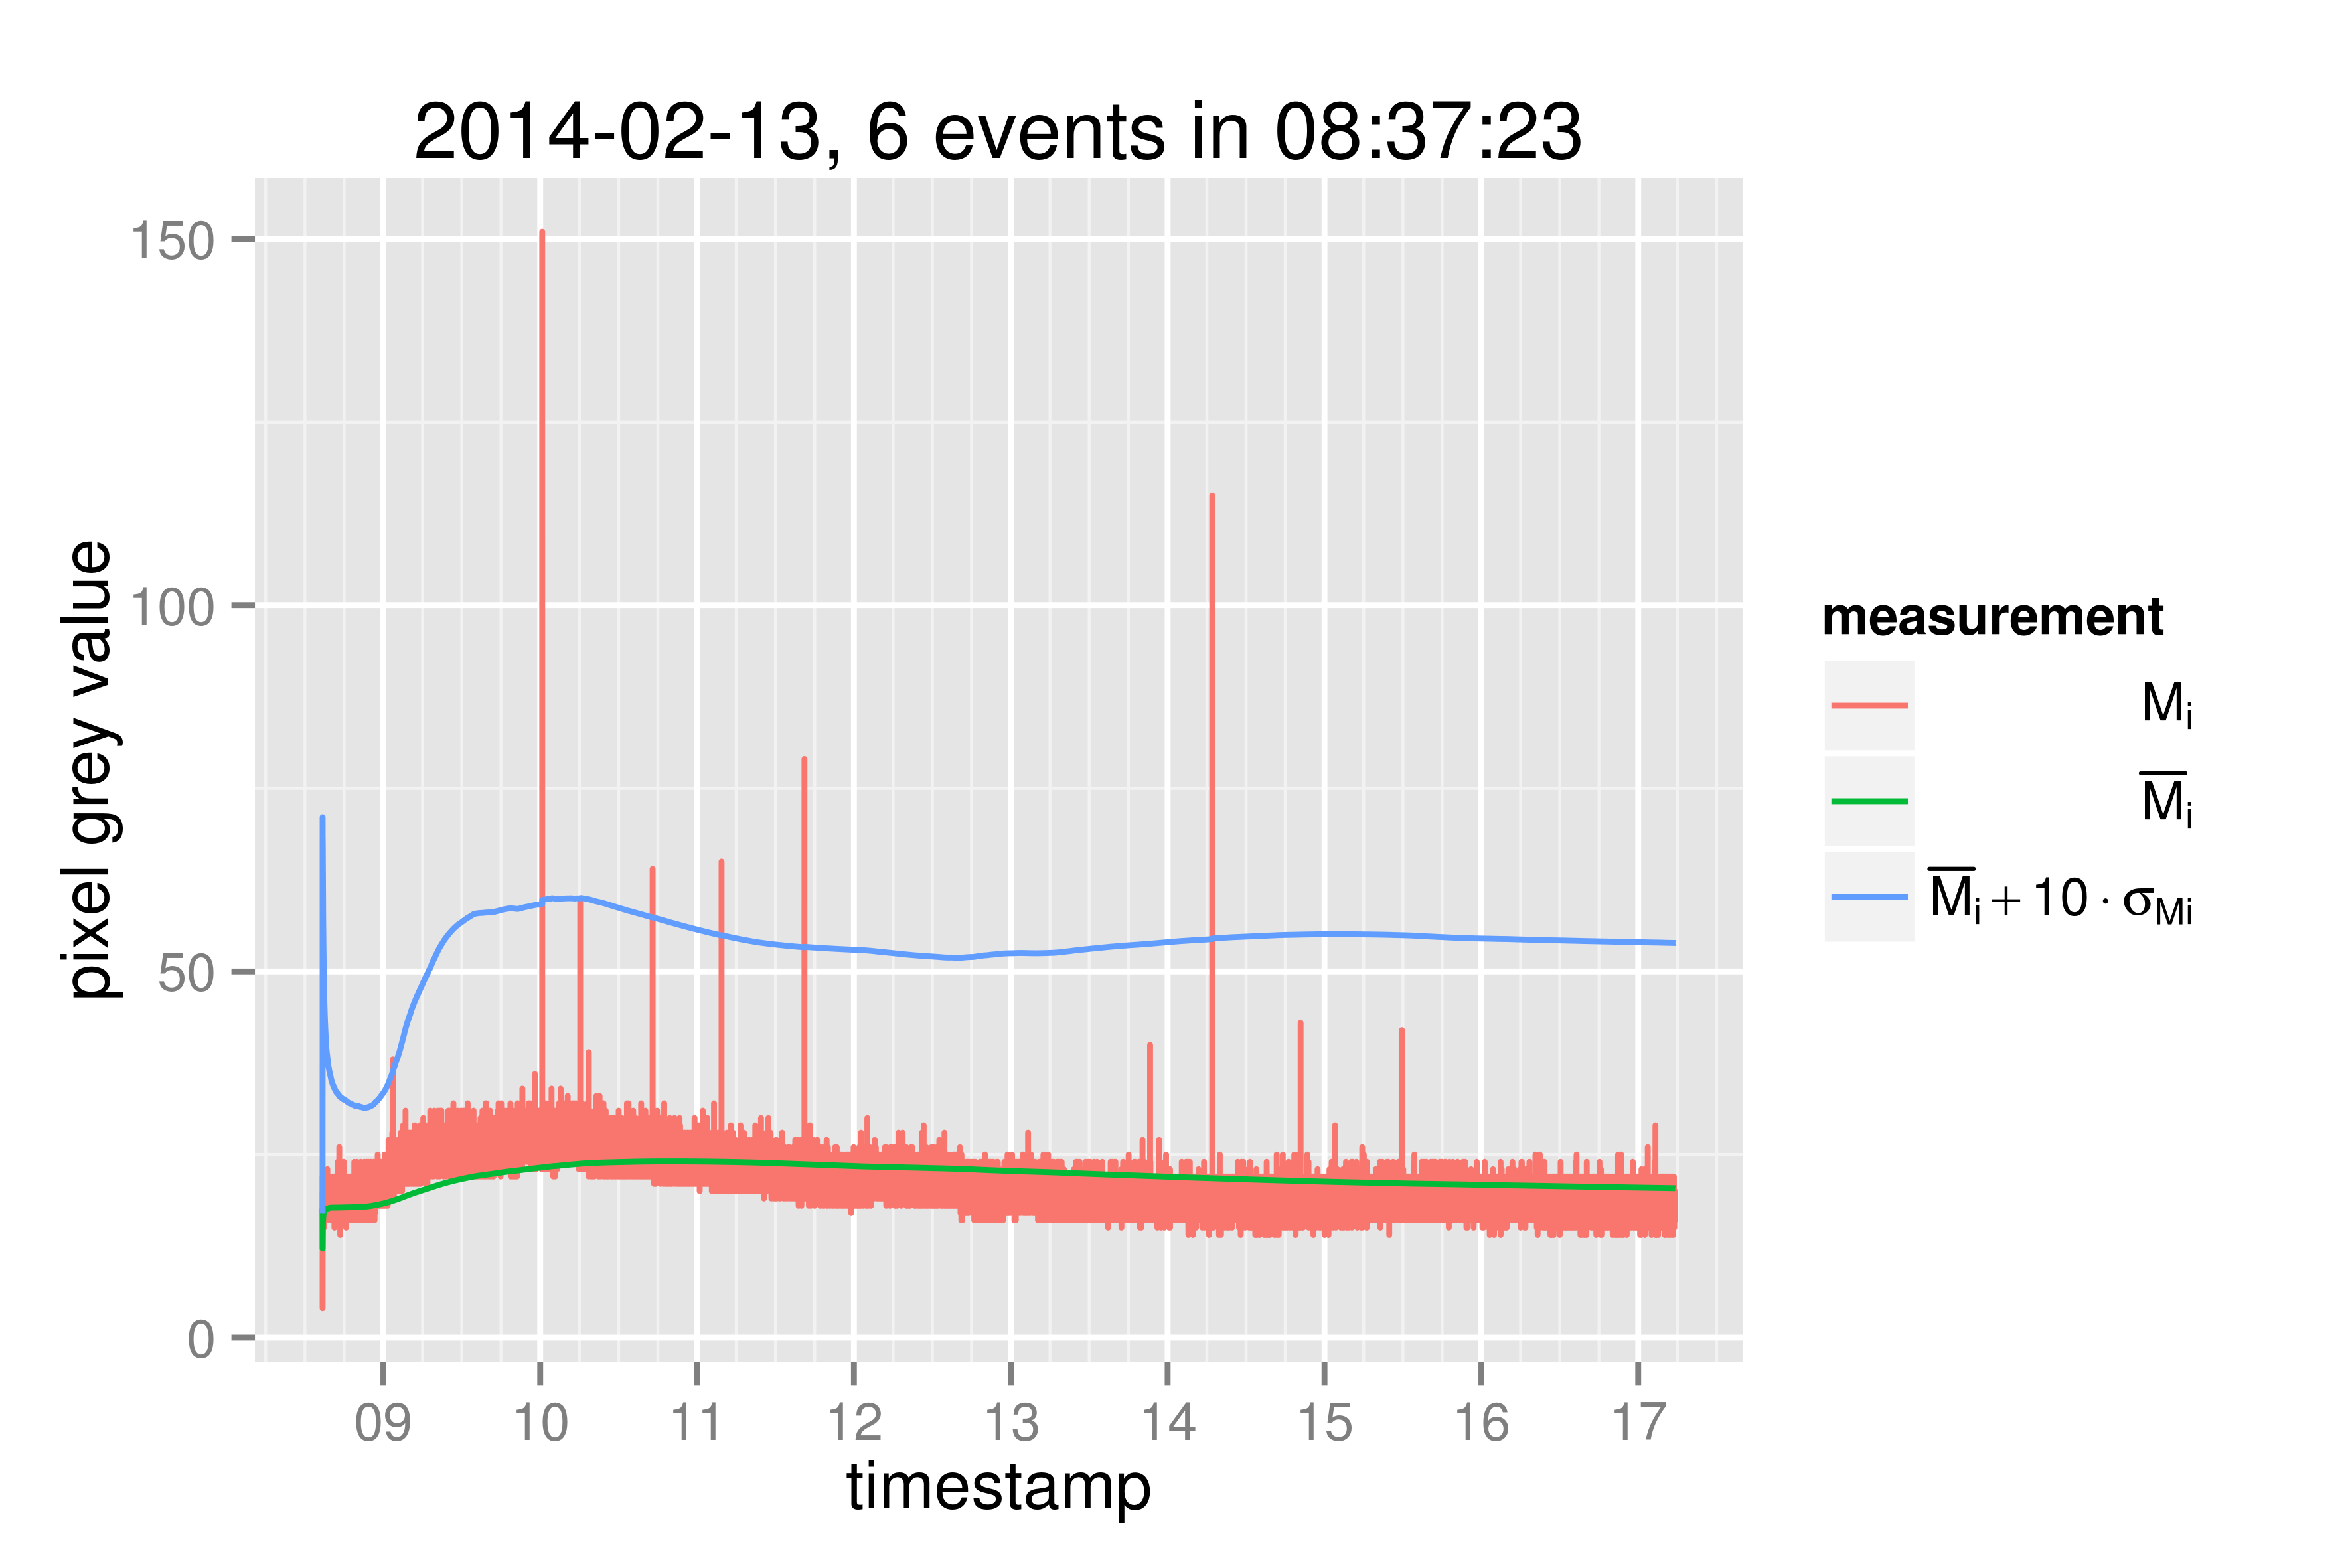
\includegraphics{20140213.png}
  \caption{Data collected using formula \ref{eq:3} with $n=10$.}\label{fig:4}
\end{figure}

\begin{figure}[h!]
  \centering
  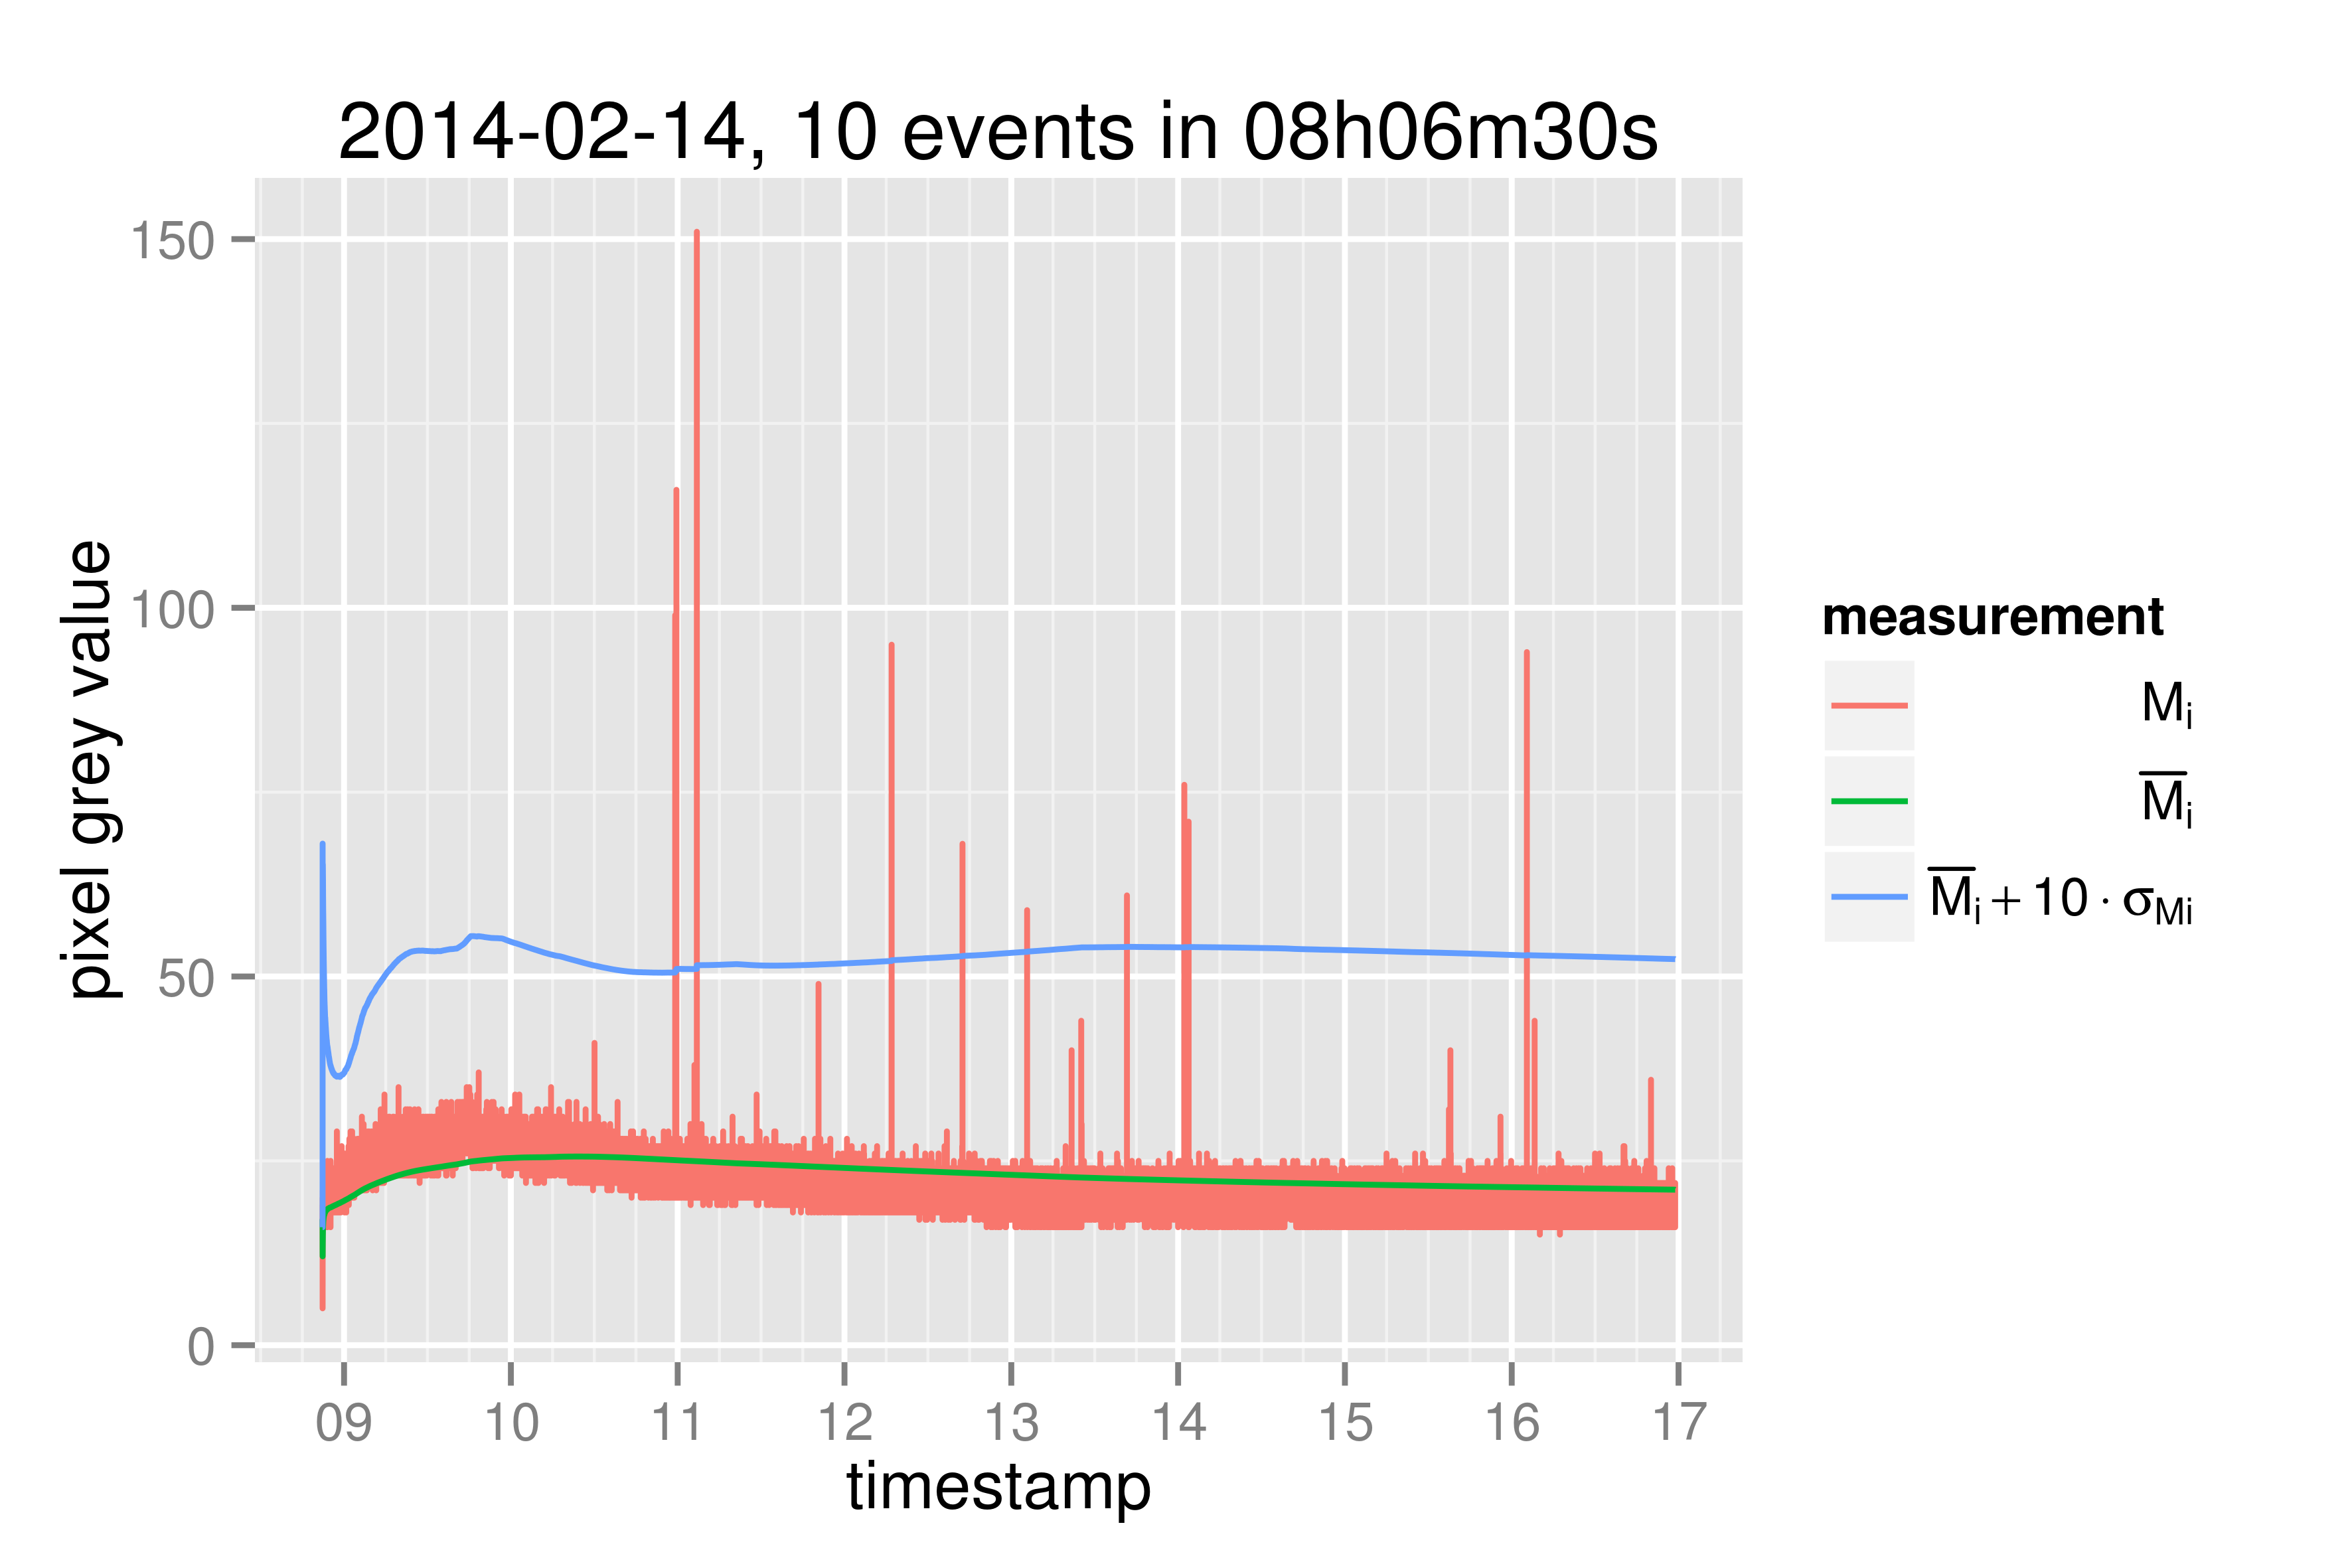
\includegraphics{20140214.png}
  \caption{Data collected using formula \ref{eq:3} with $n=10$.}
\end{figure}

\begin{figure}[h!]
  \centering
  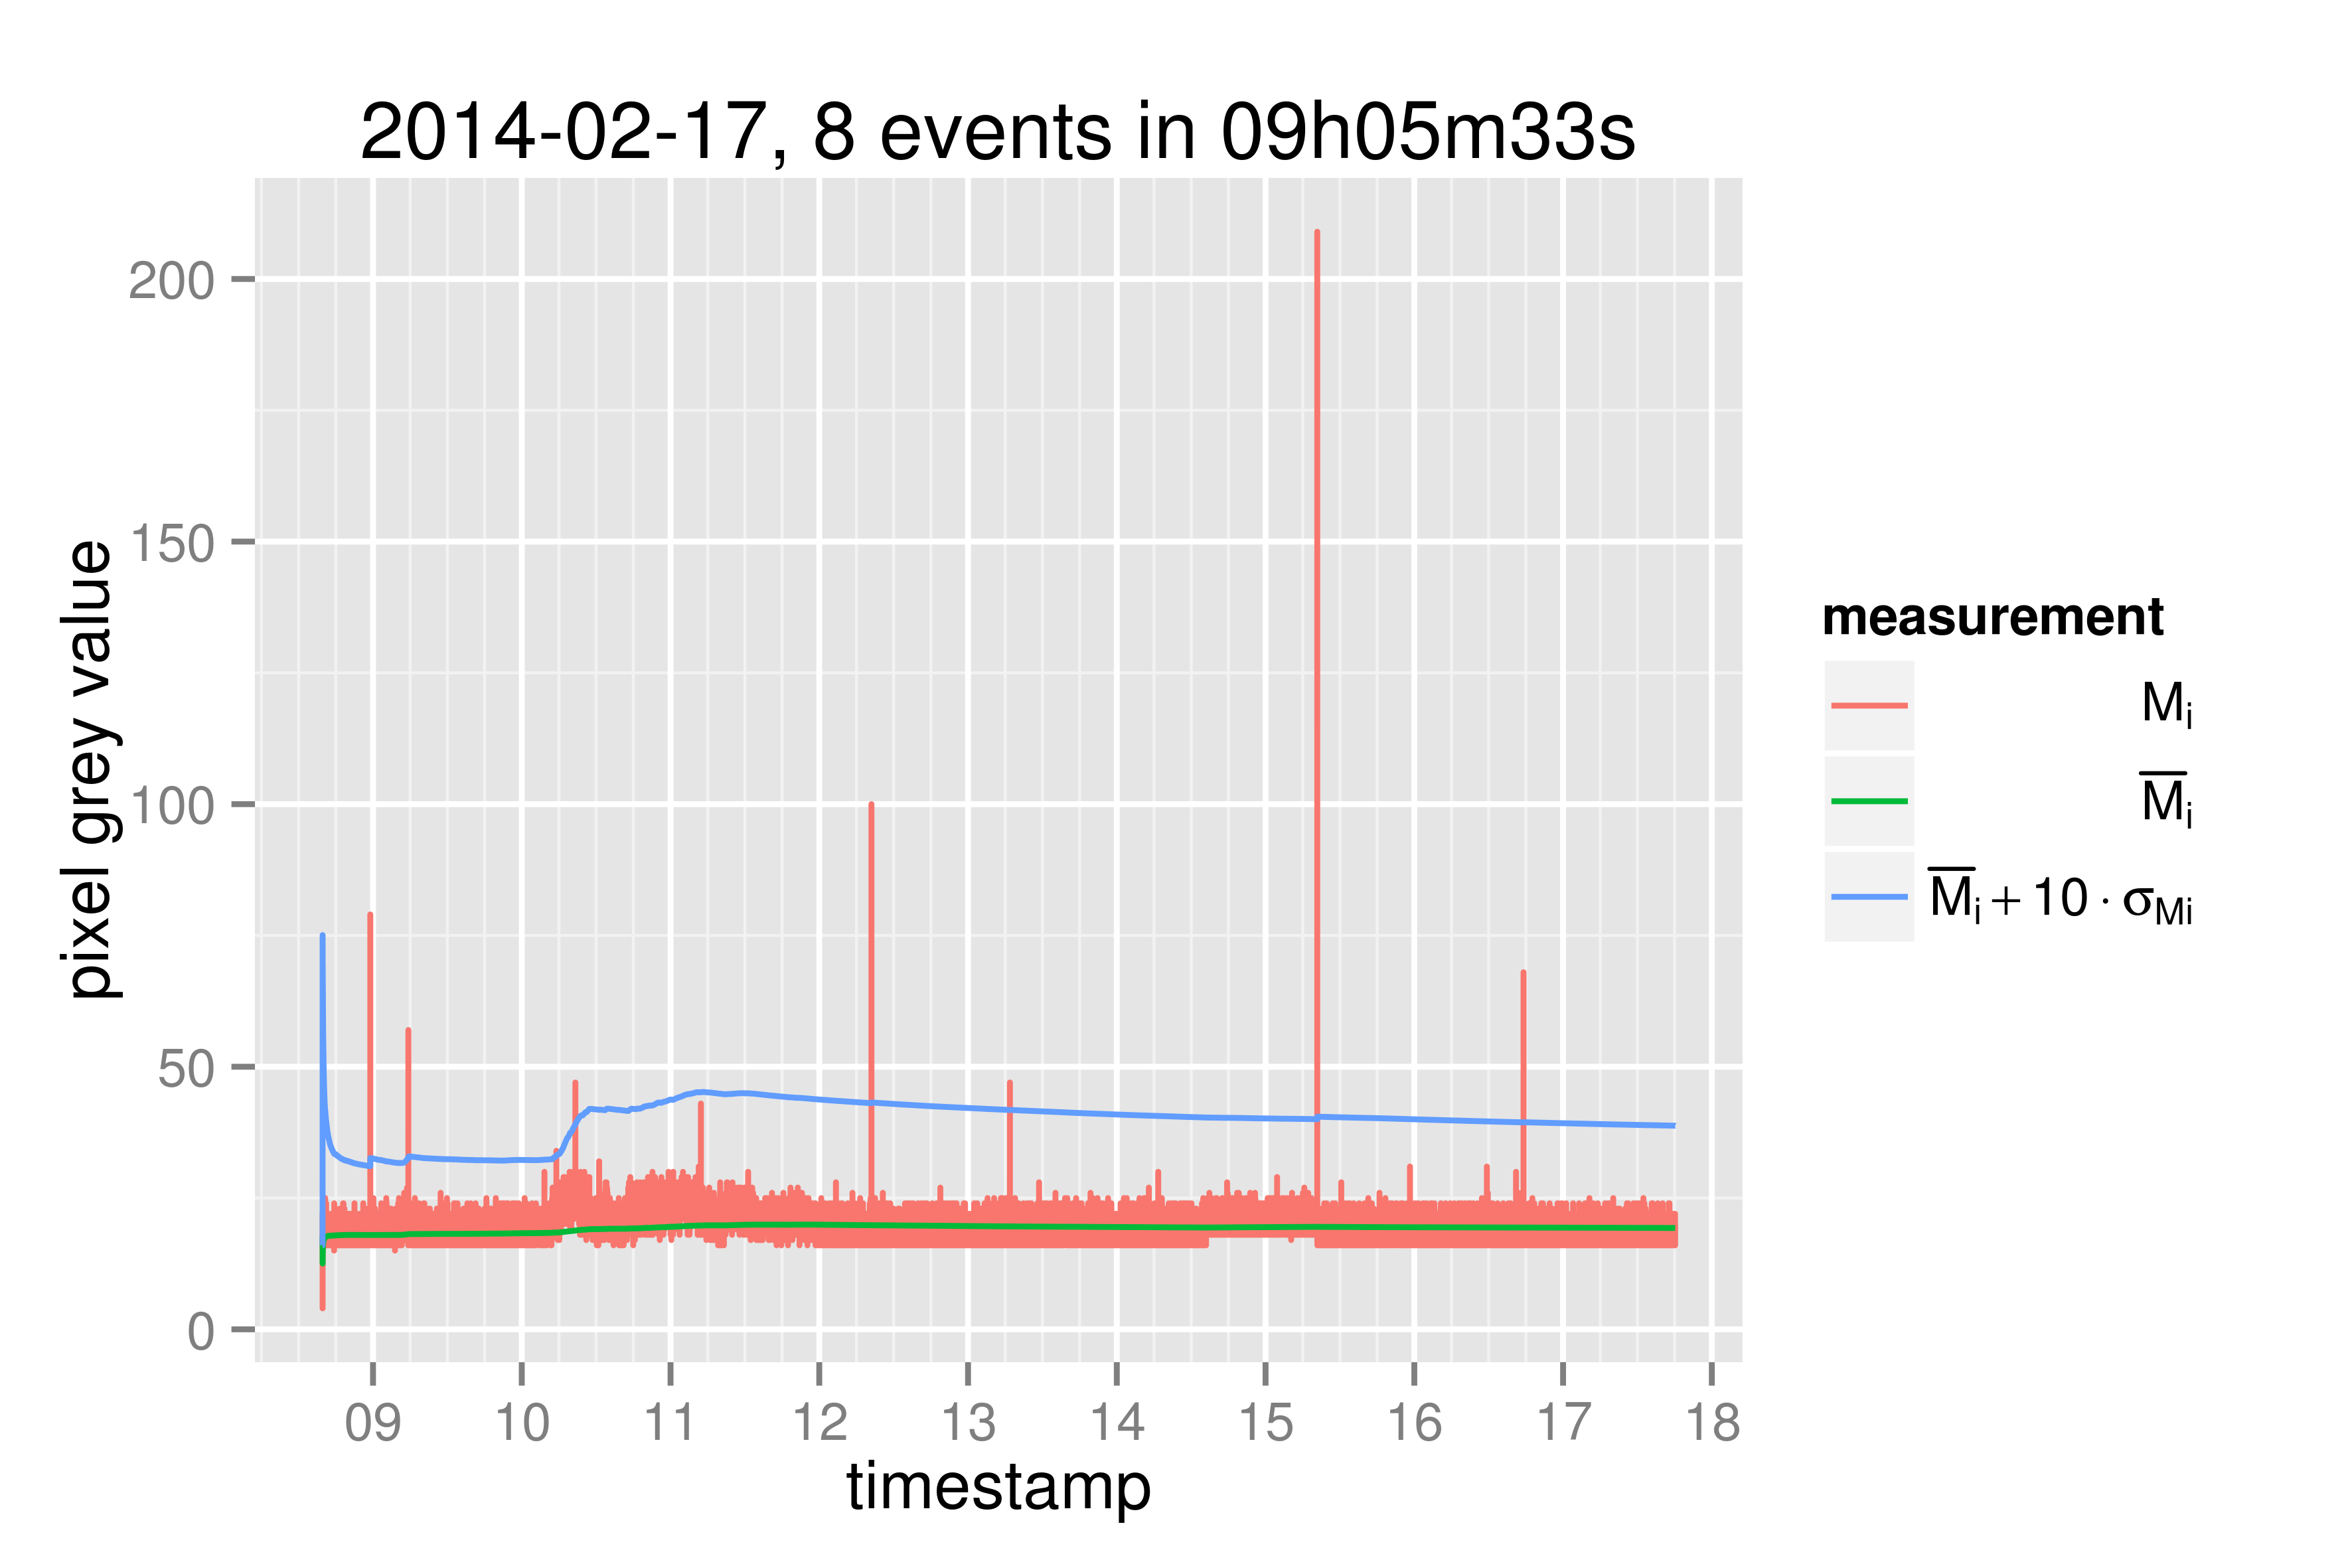
\includegraphics{20140217.png}
  \caption{Data collected using formula \ref{eq:3} with $n=10$.}
\end{figure}

\begin{figure}[h!]
  \centering
  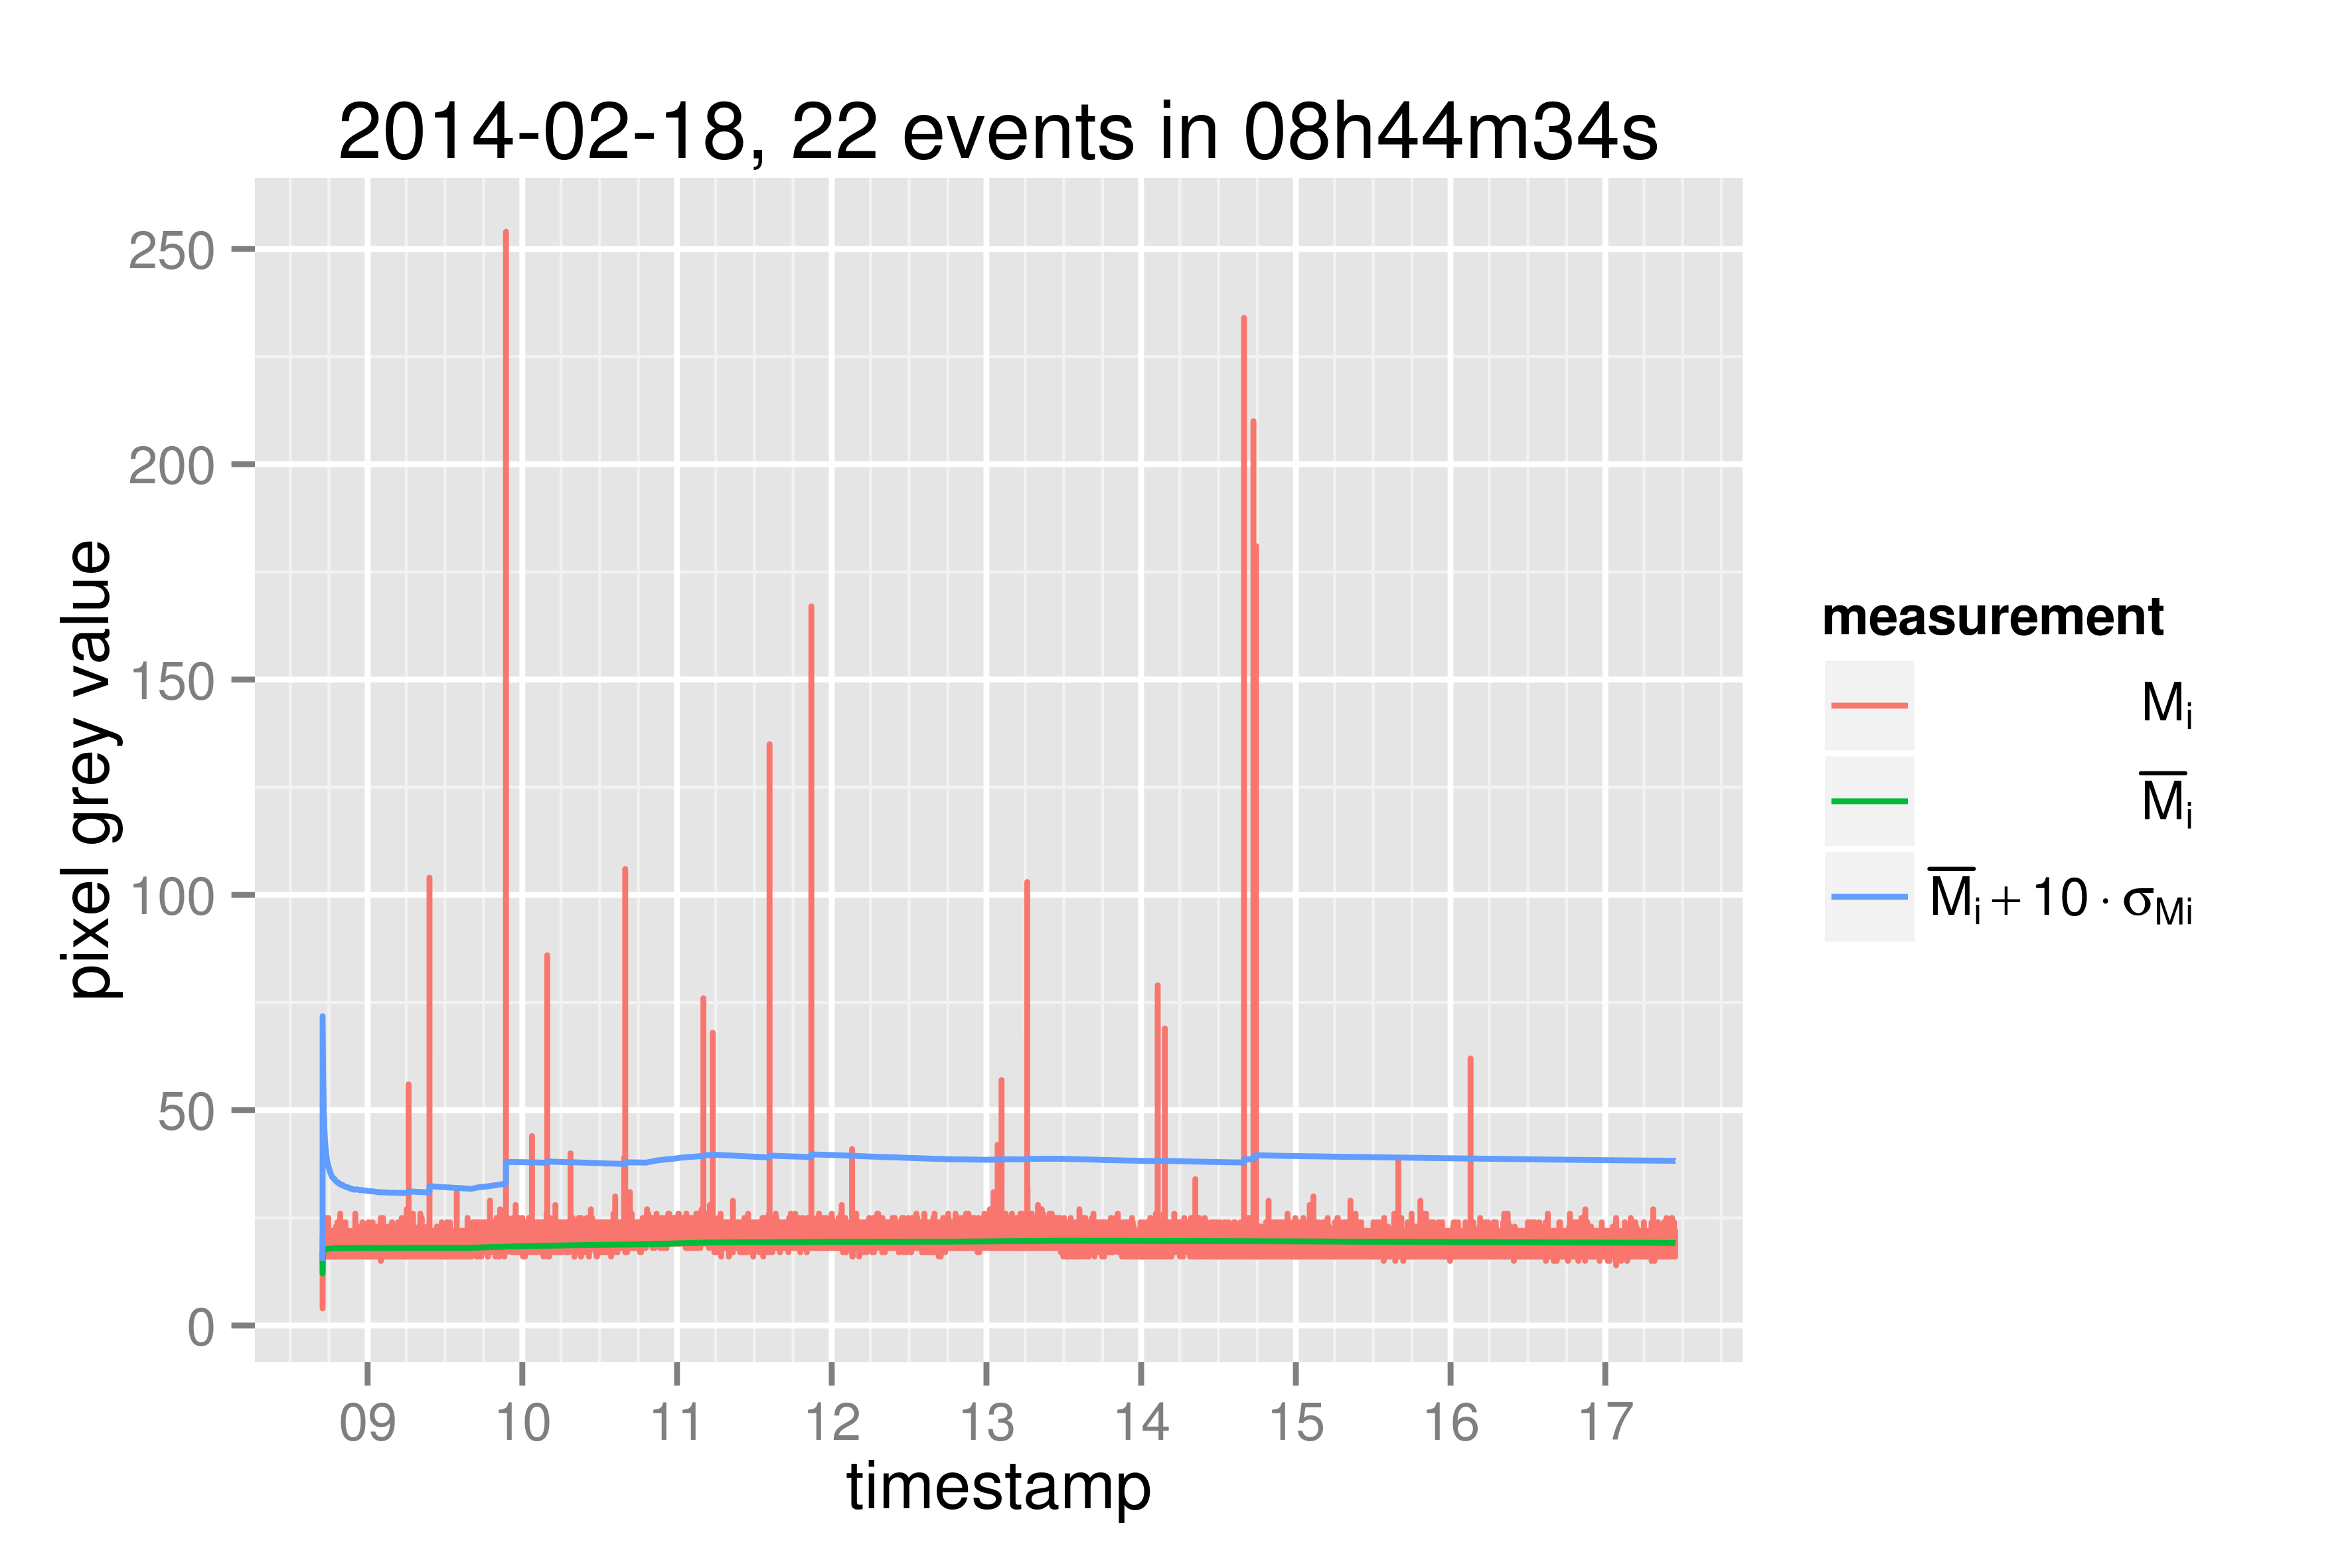
\includegraphics{20140218.png}
  \caption{Data collected using formula \ref{eq:3} with $n=10$.}
\end{figure}

\begin{figure}[h!]
  \centering
  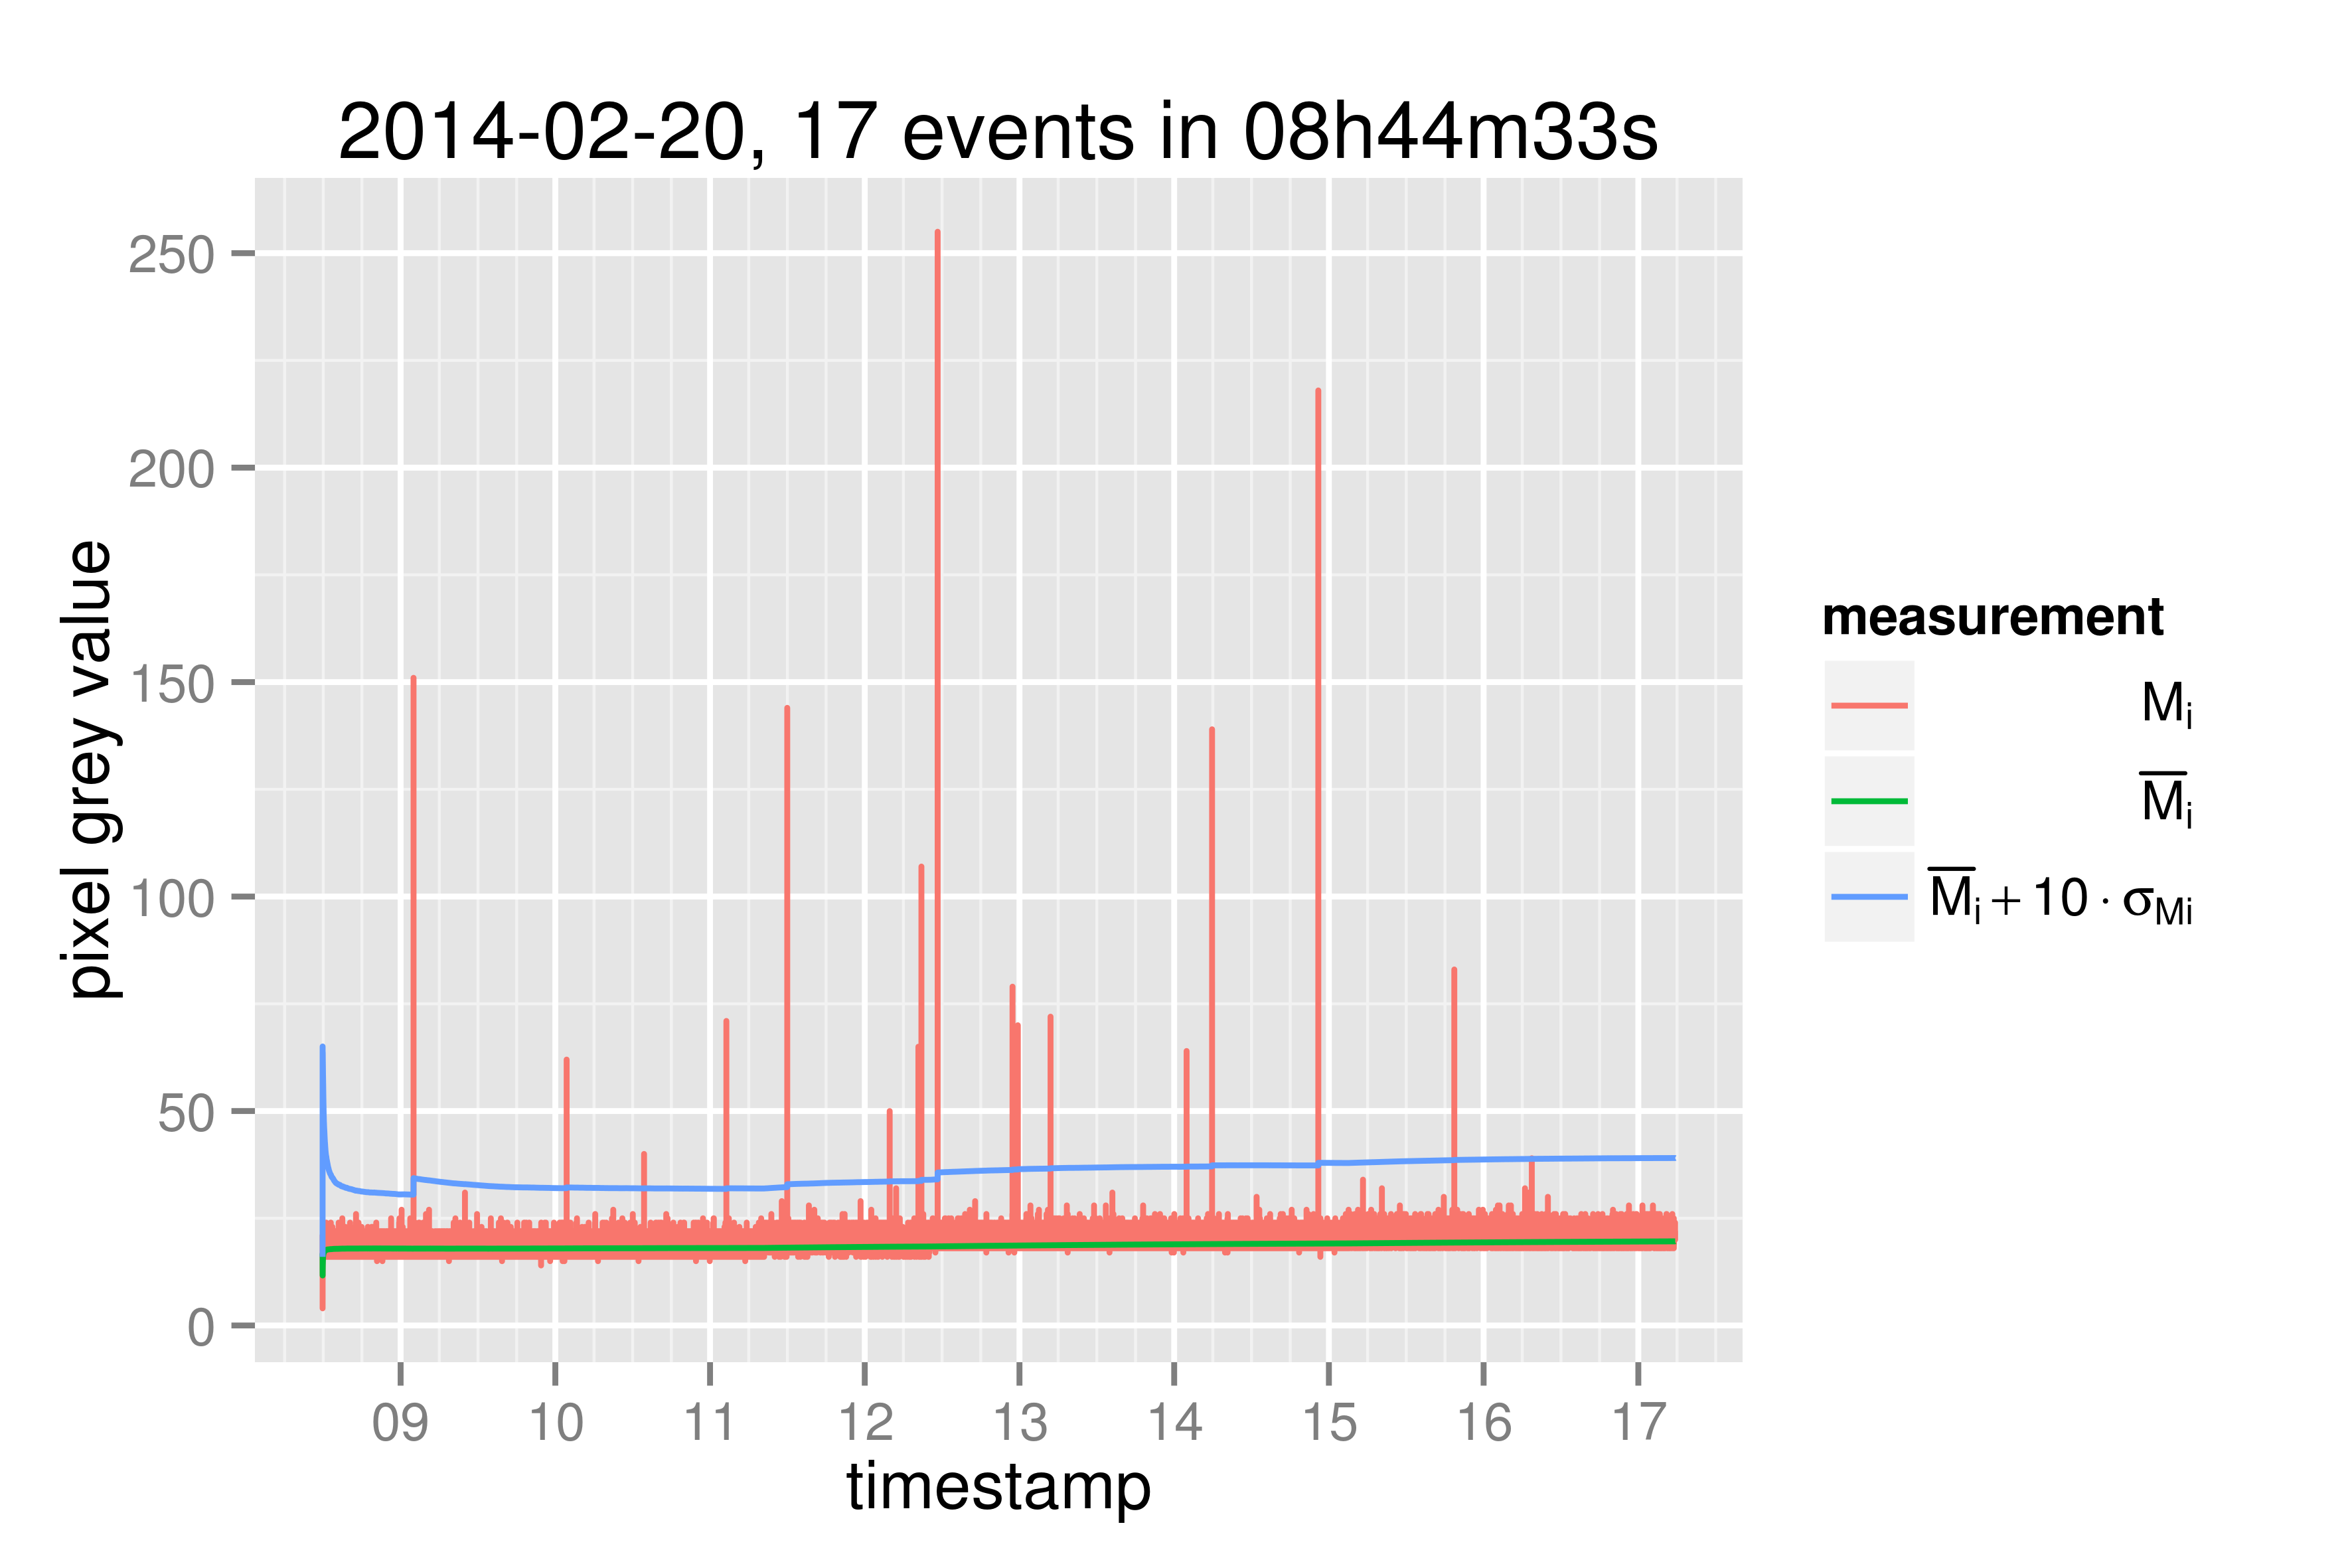
\includegraphics{20140220.png}
  \caption{Data collected using formula \ref{eq:3} with $n=10$.}
\end{figure}

\begin{figure}[h!]
  \centering
  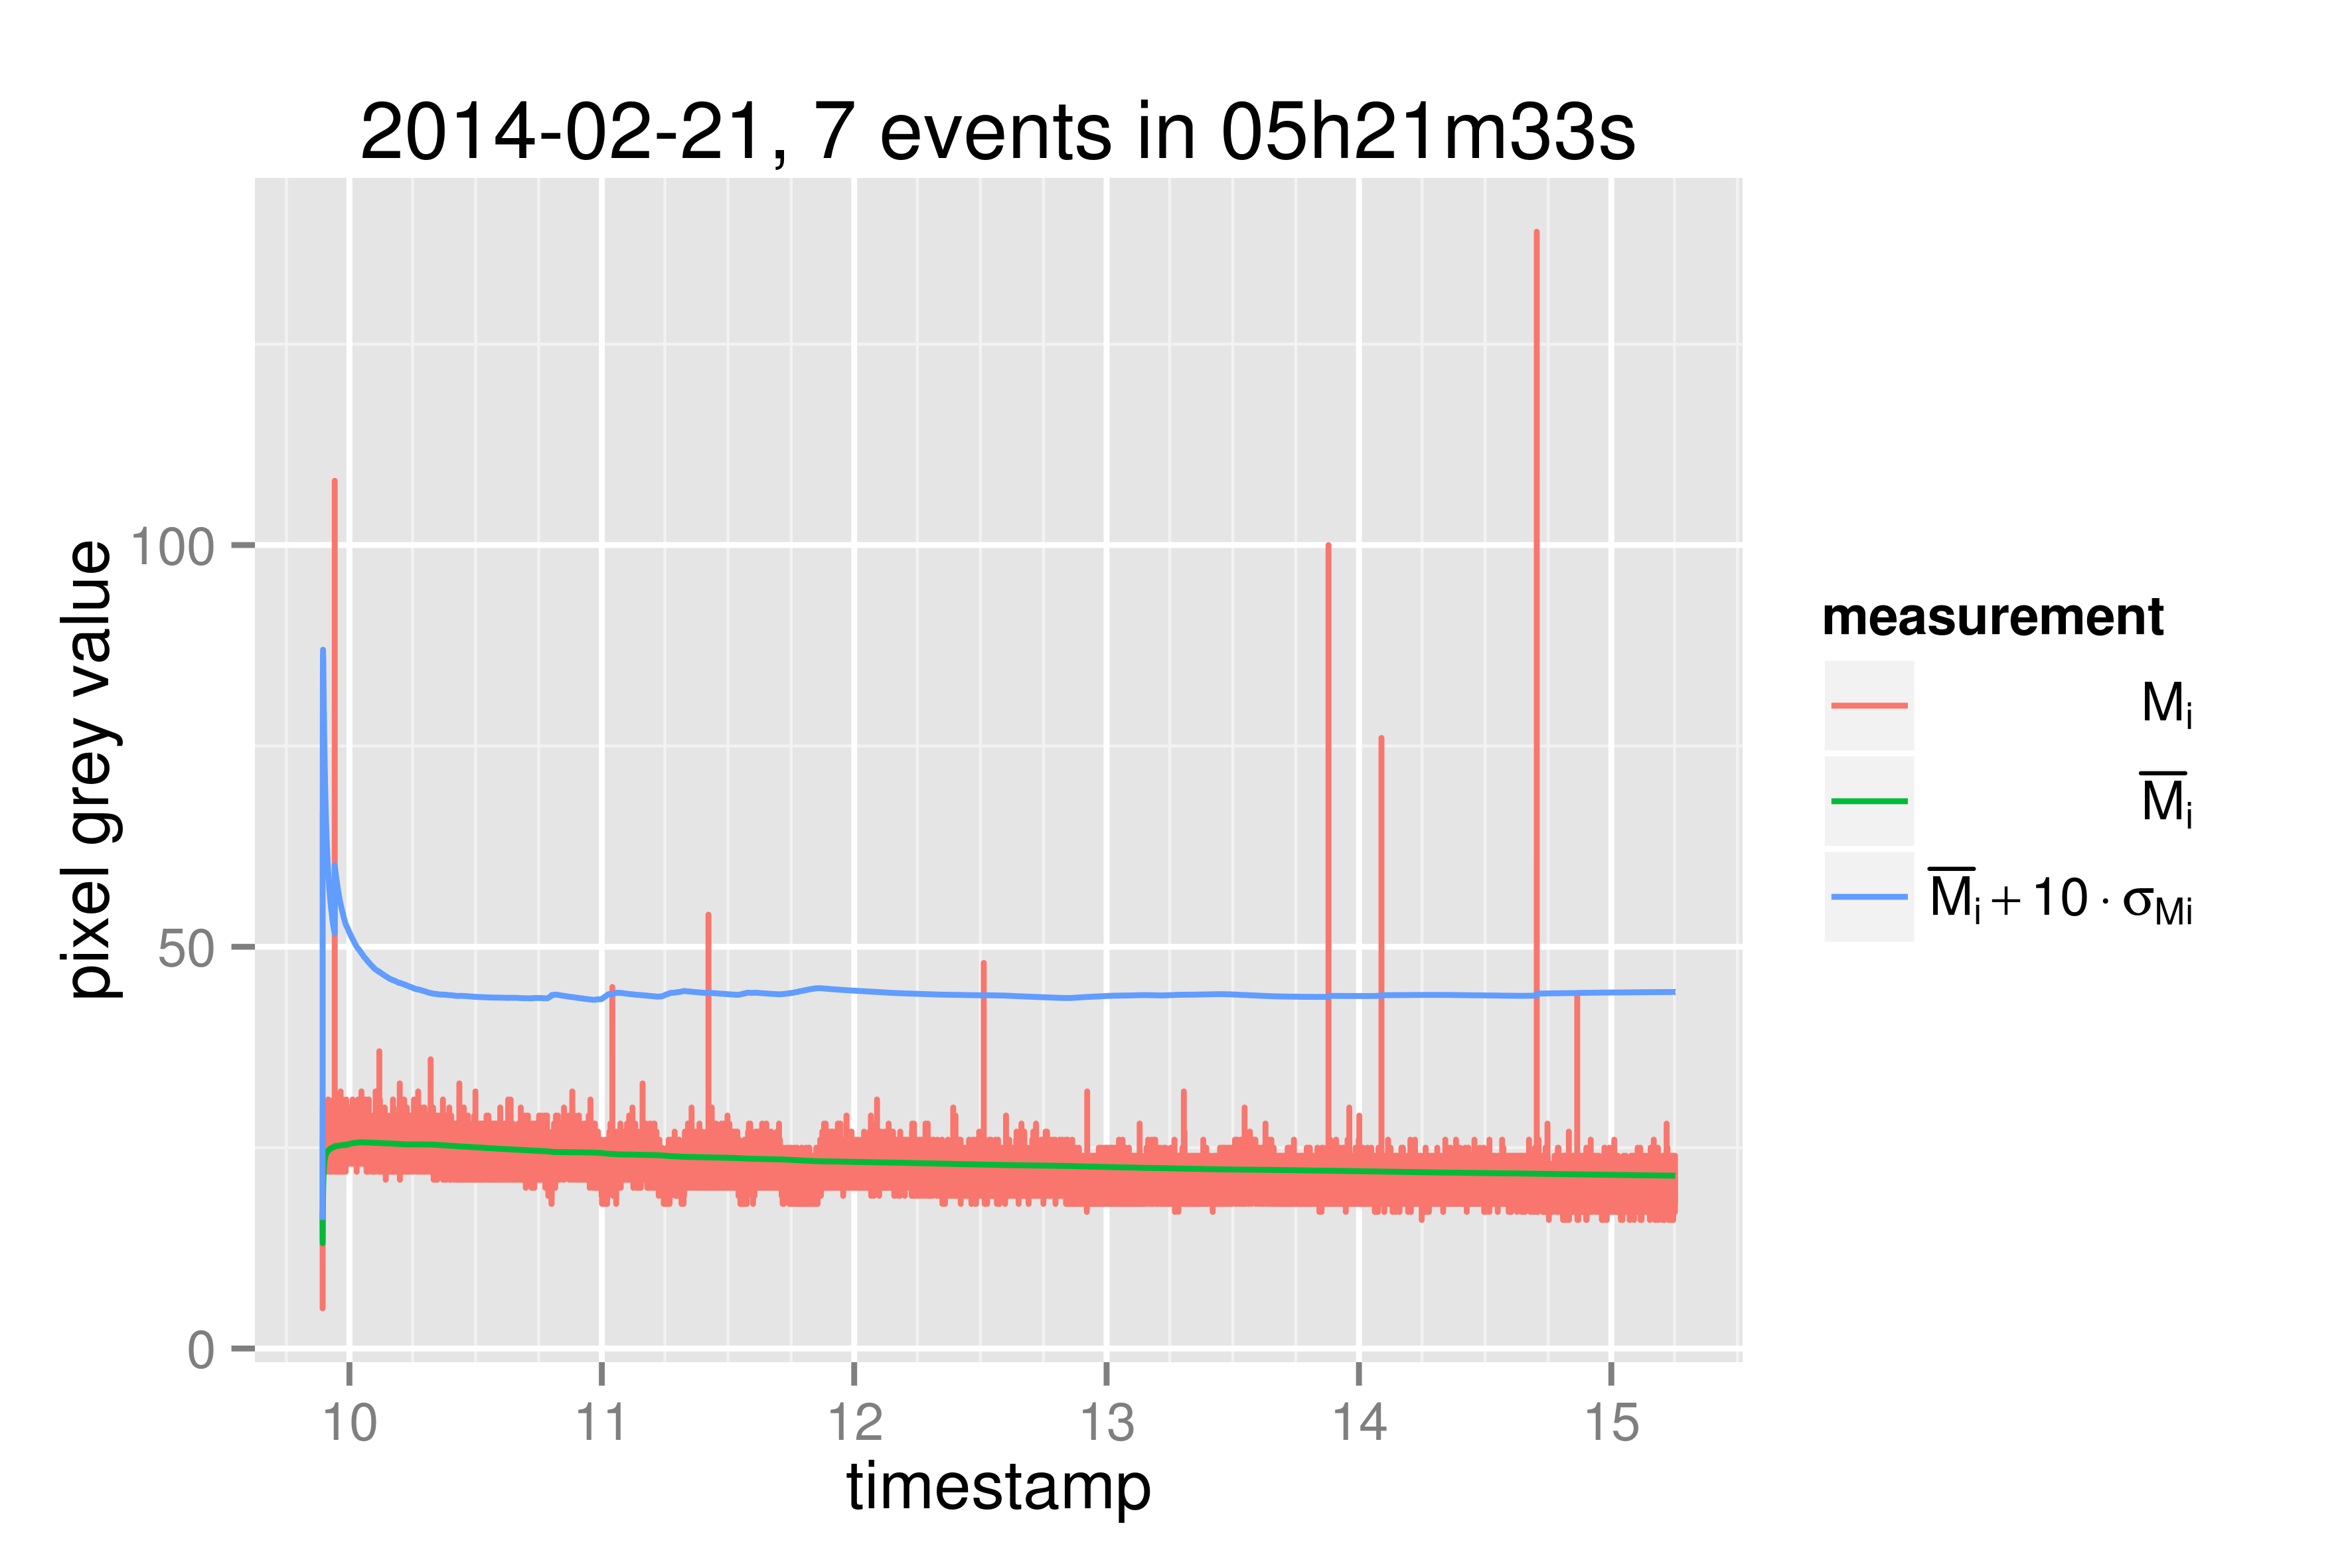
\includegraphics{20140221.png}
  \caption{Data collected using formula \ref{eq:3} with $n=10$.}
\end{figure}

\begin{figure}[h!]
  \centering
  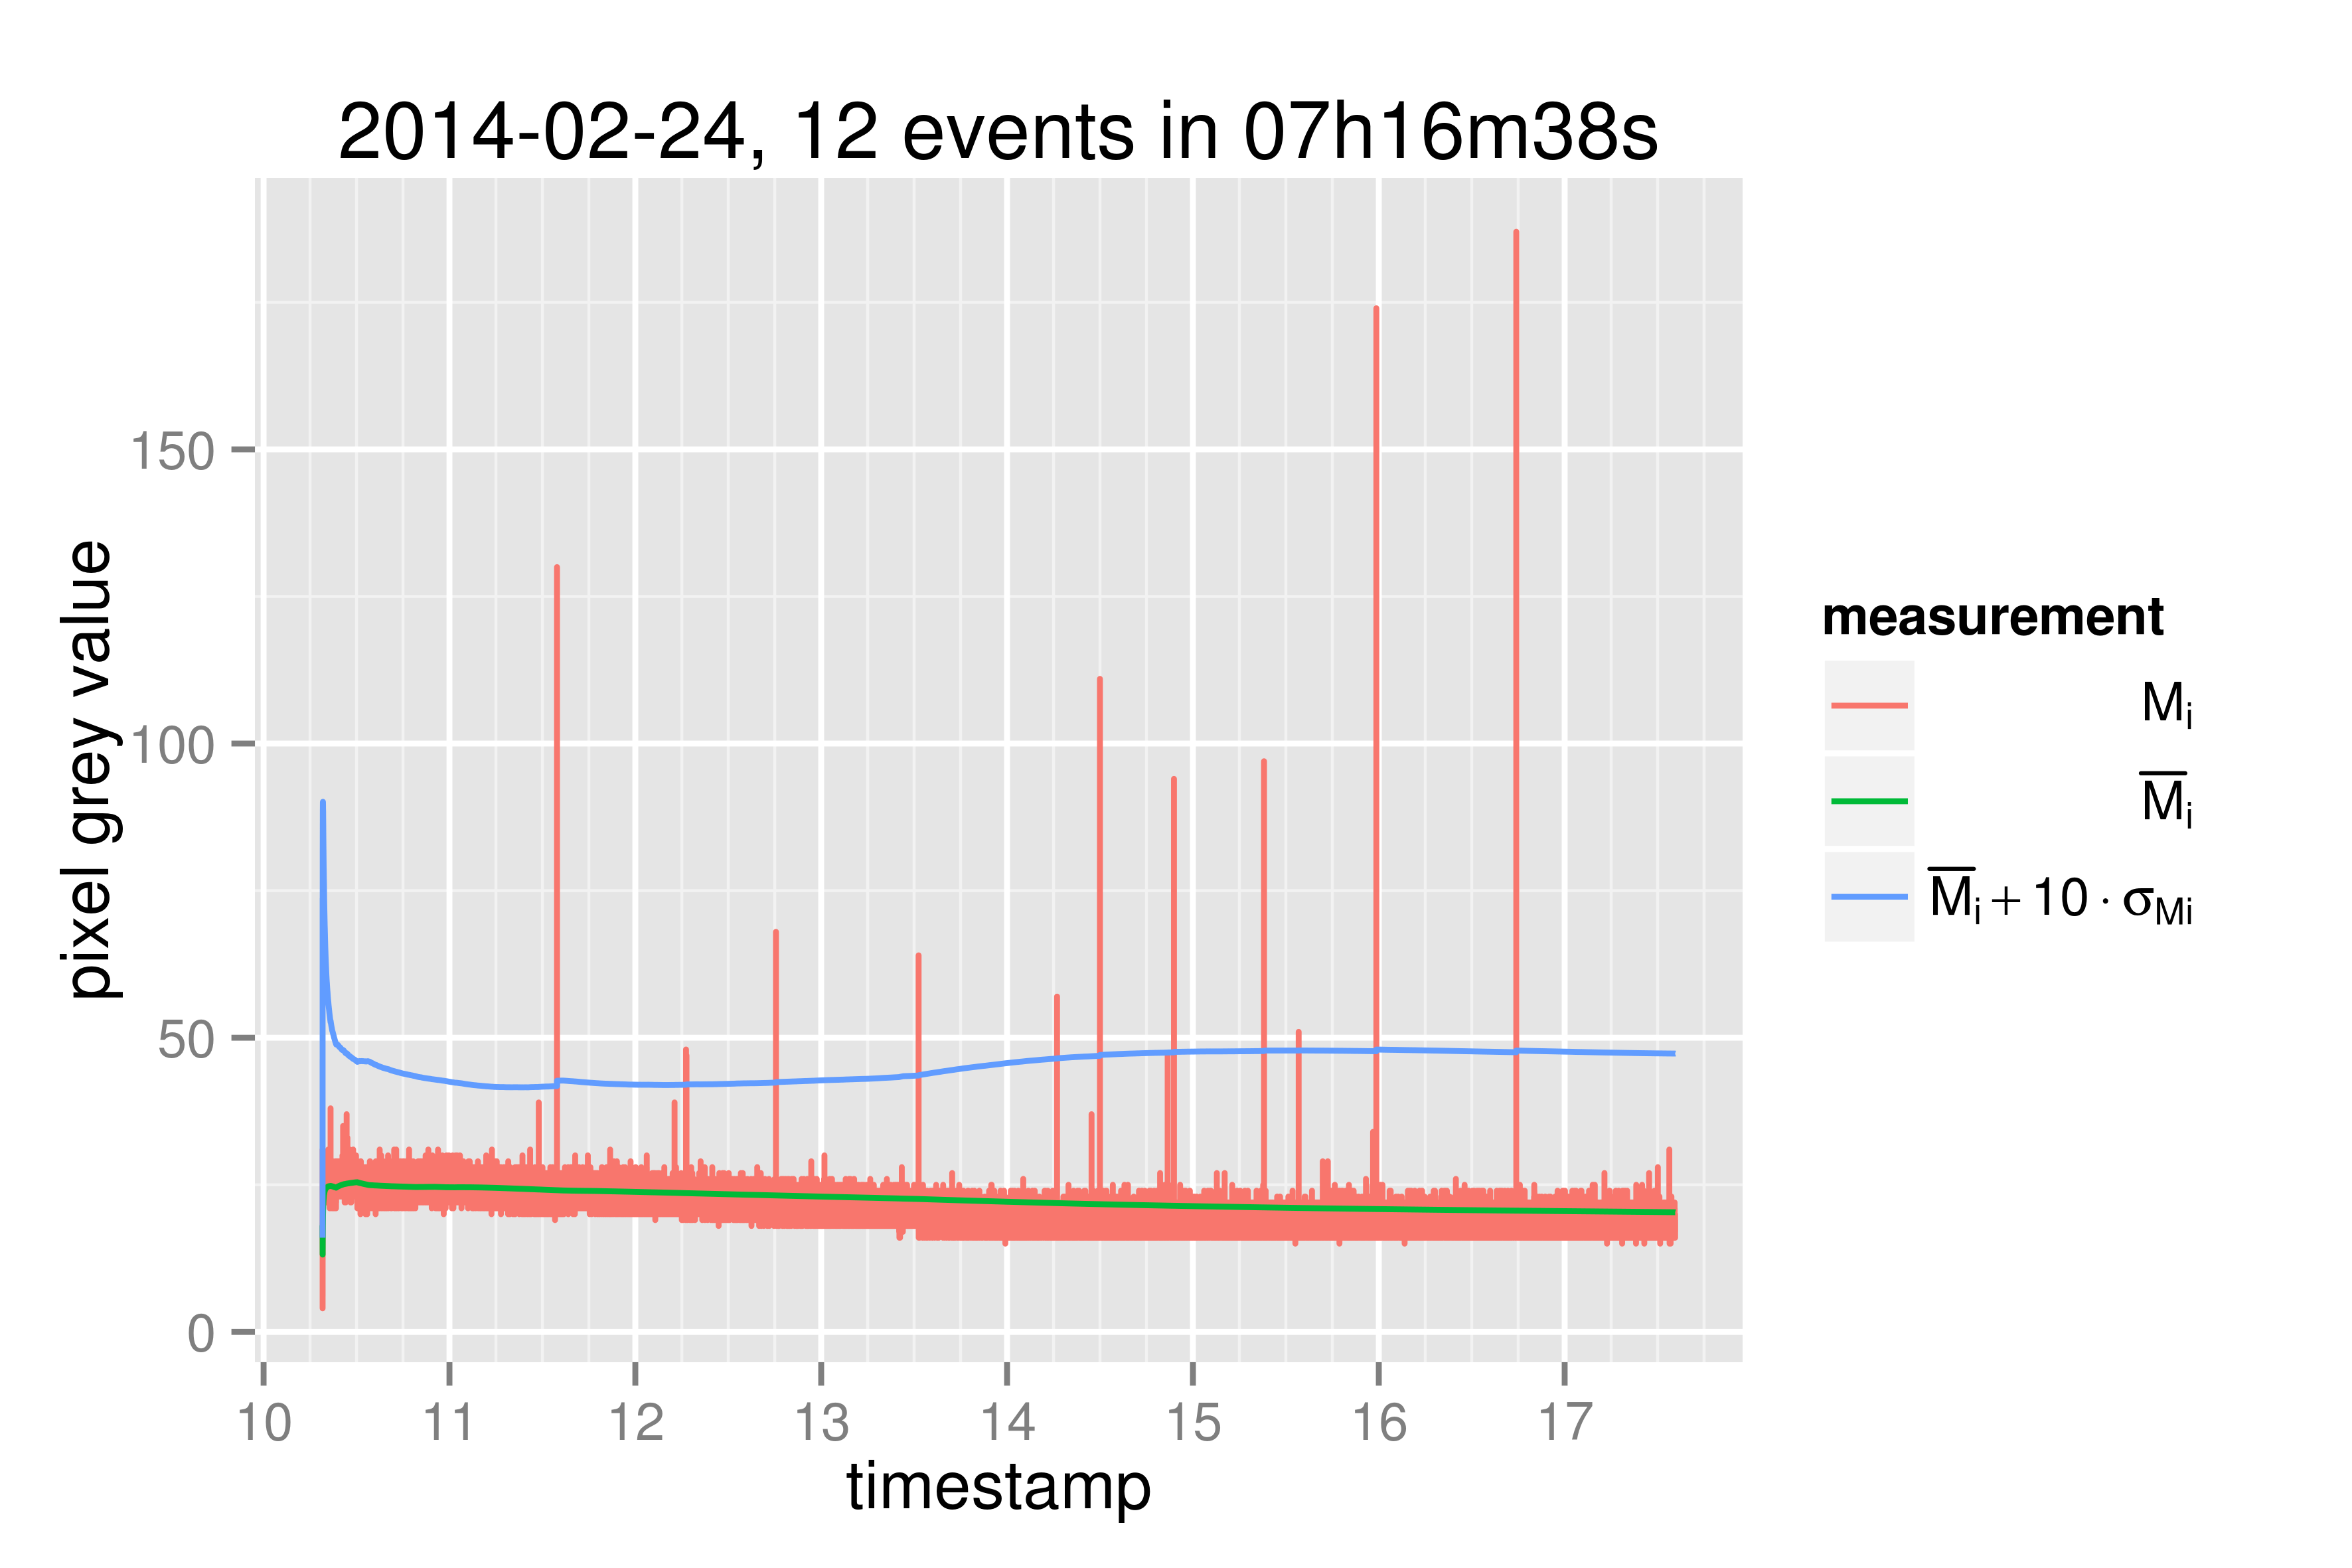
\includegraphics{20140224.png}
  \caption{Data collected using formula \ref{eq:3} with $n=10$.}
\end{figure}

\begin{figure}[h!]
  \centering
  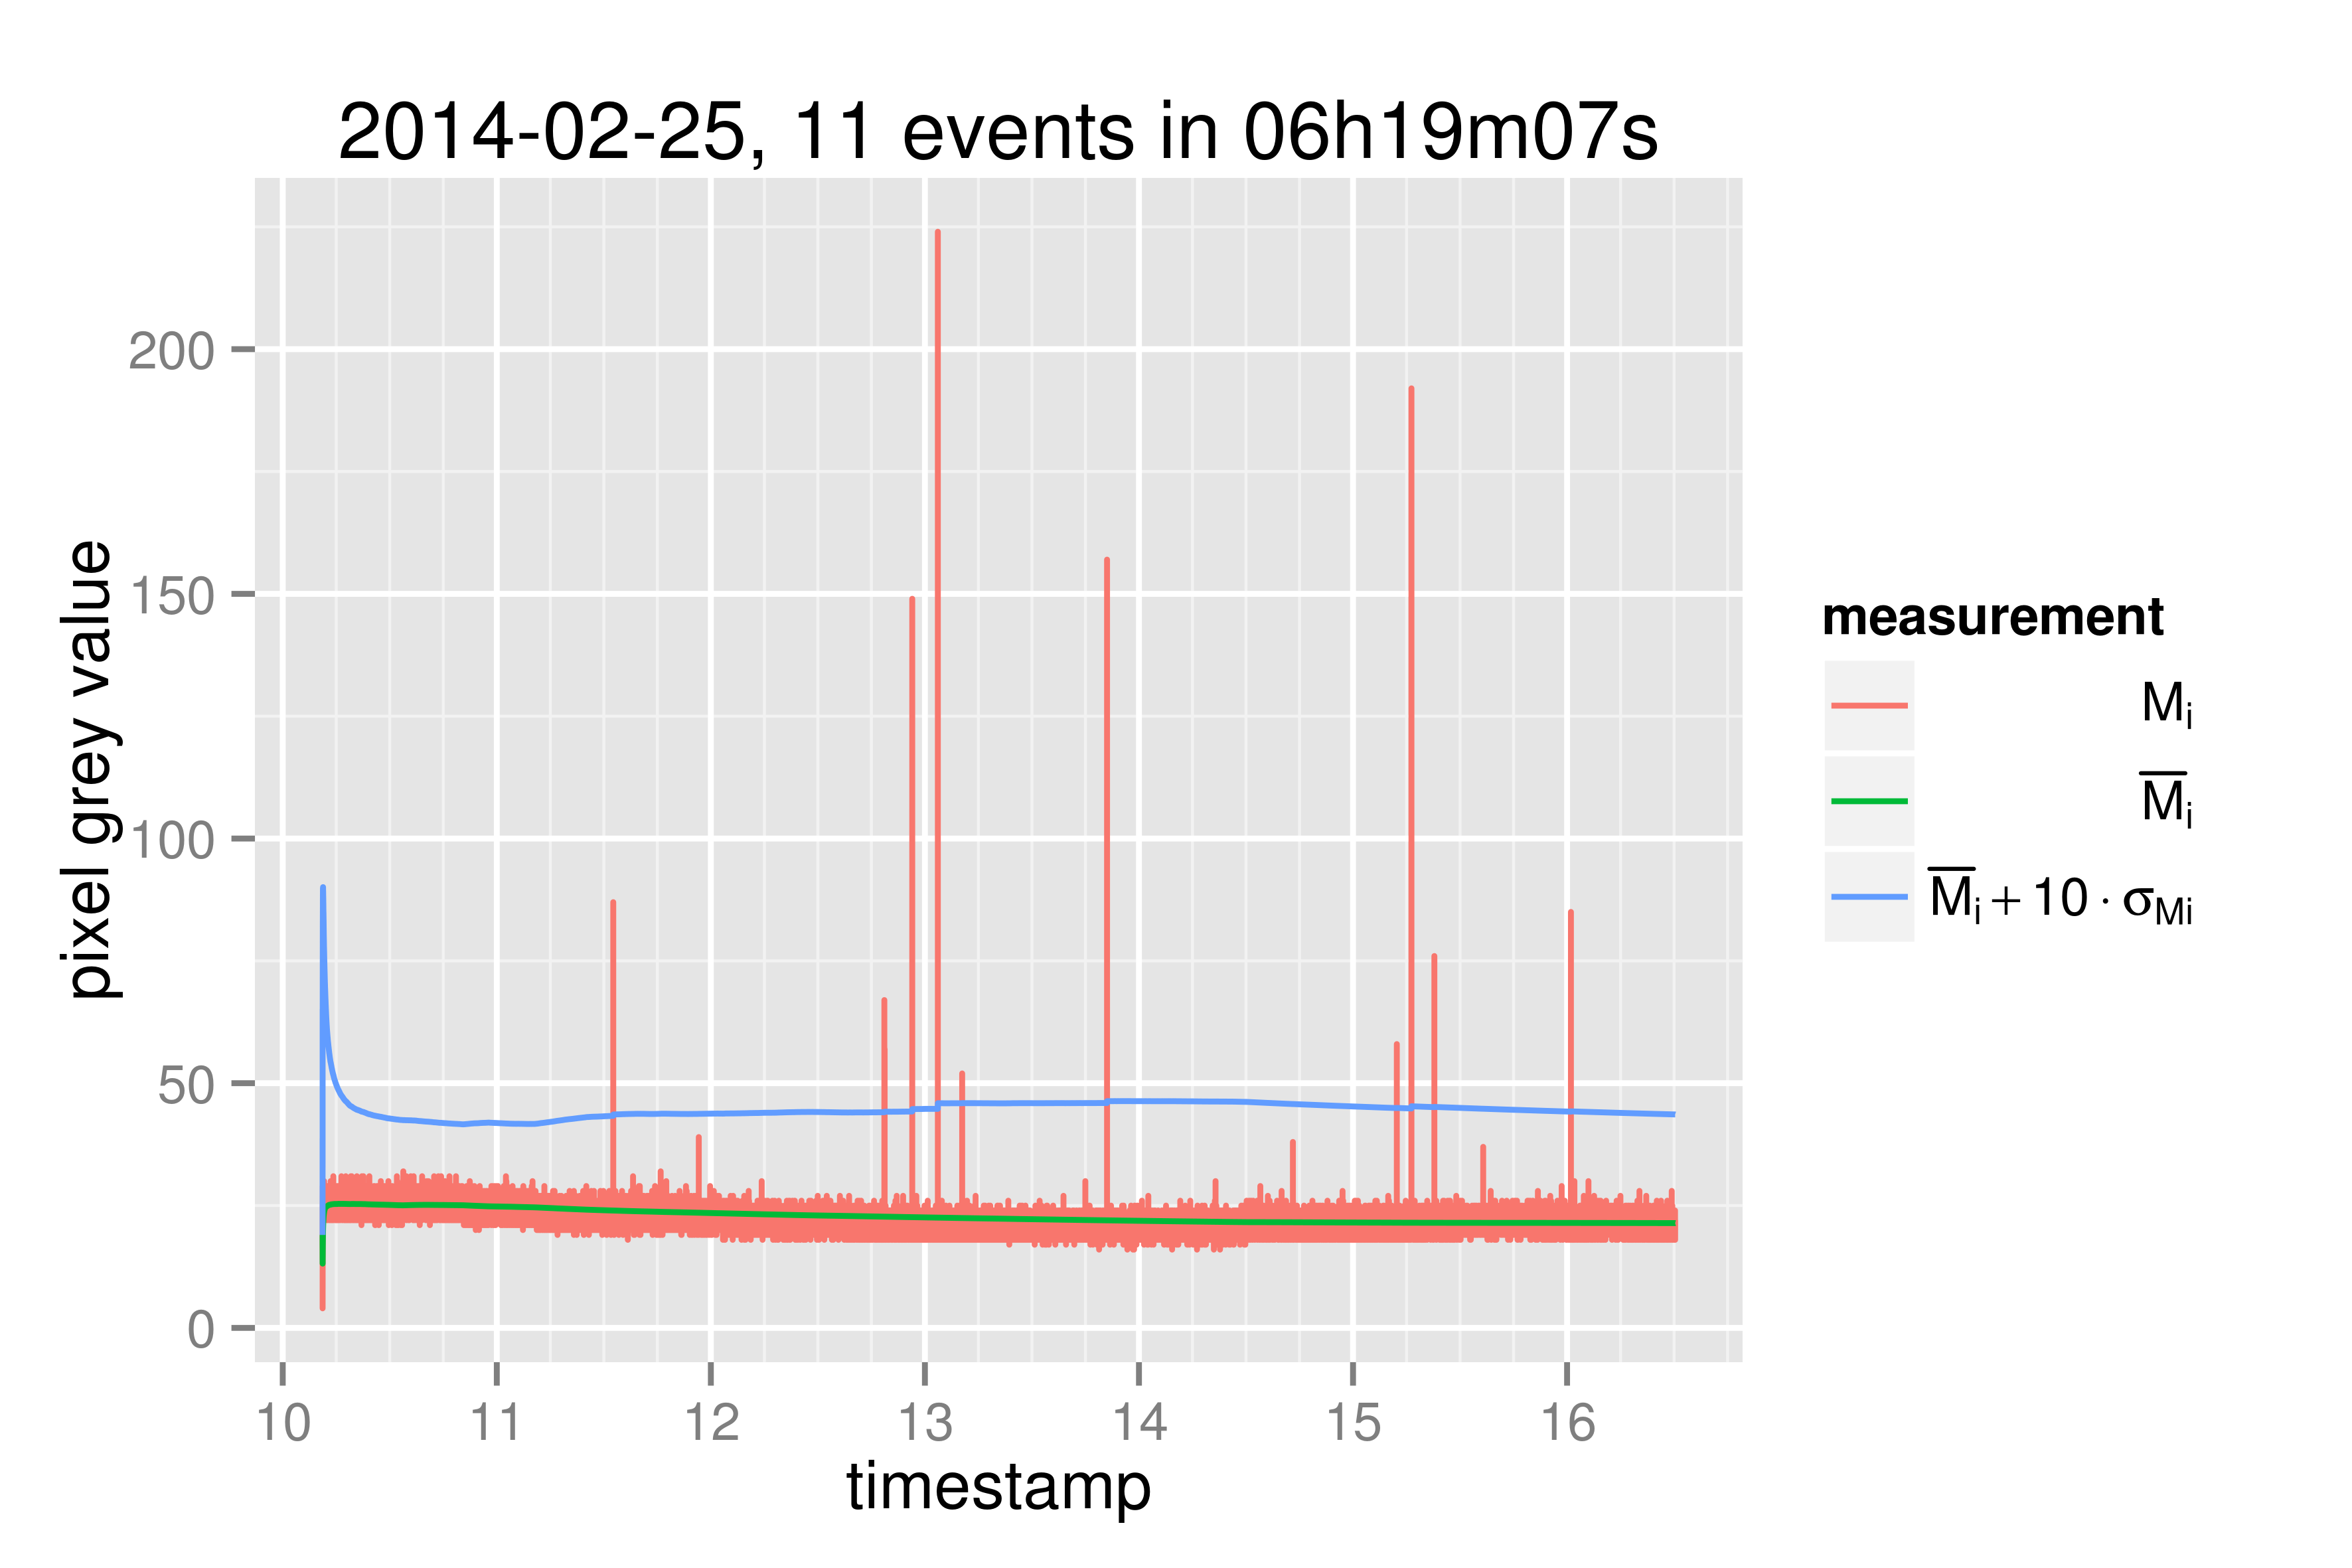
\includegraphics{20140225.png}
  \caption{Data collected using formula \ref{eq:3} with $n=10$.}
\end{figure}

\begin{figure}[h!]
  \centering
  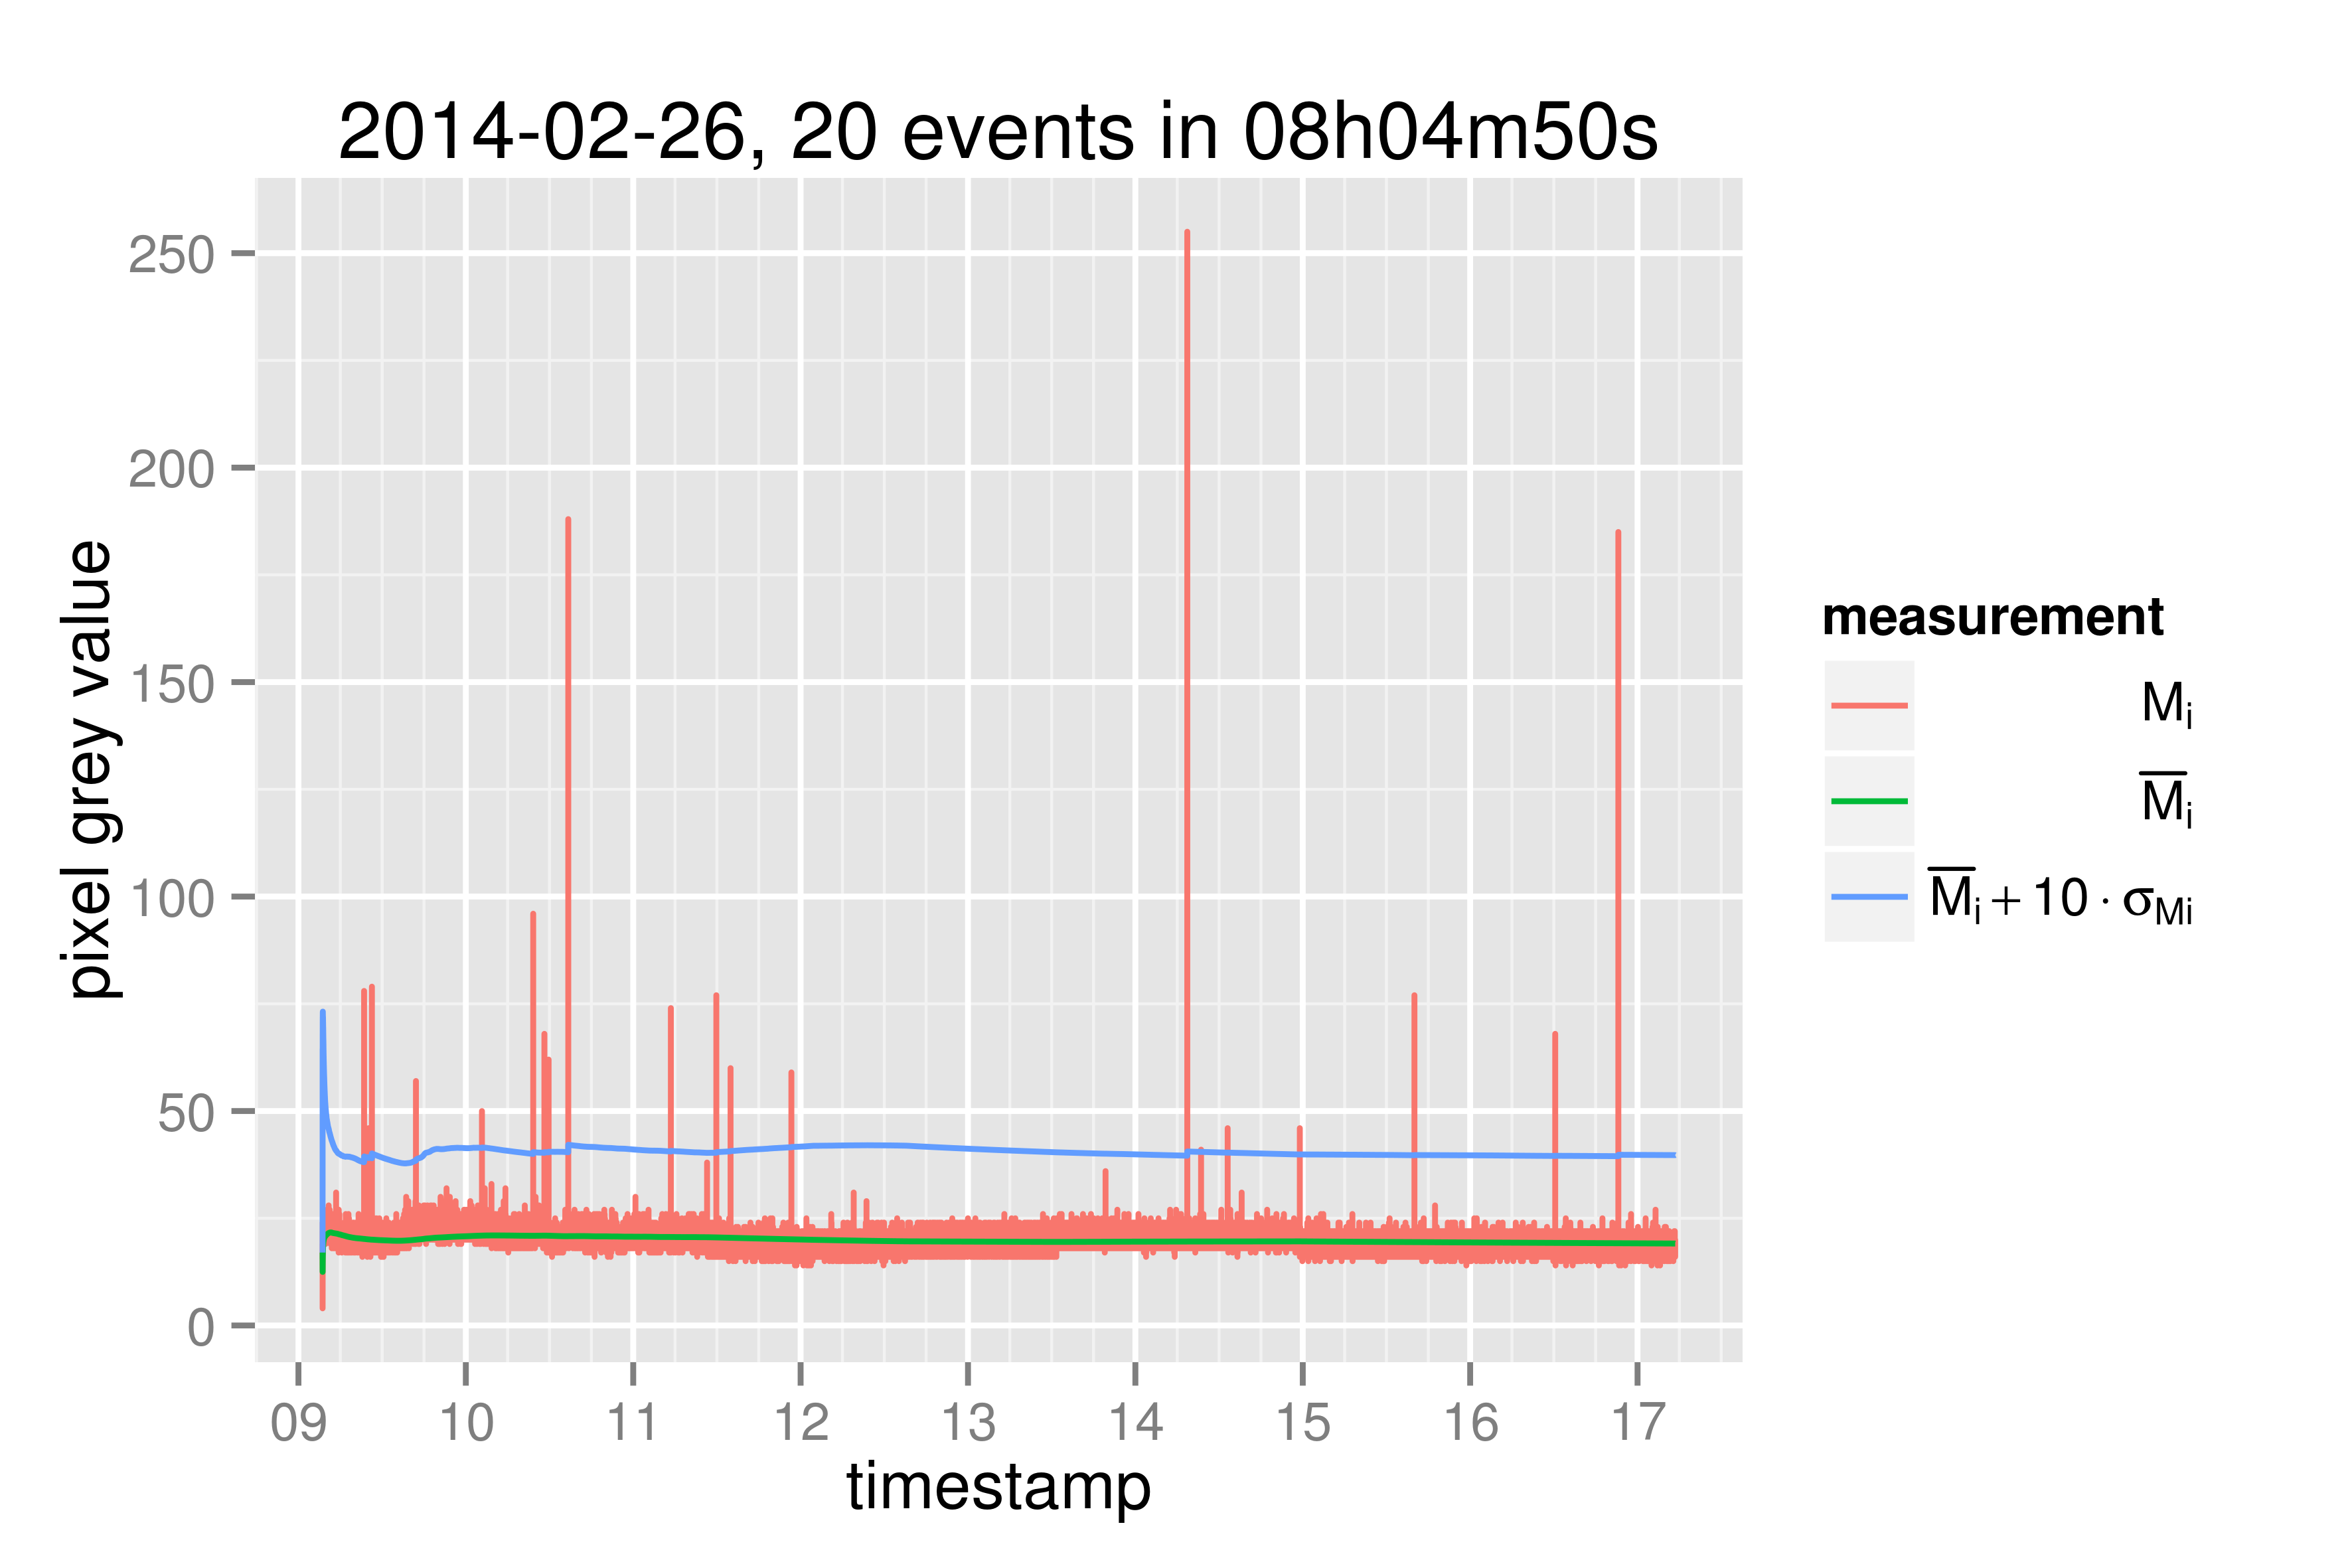
\includegraphics{20140226.png}
  \caption{Data collected using formula \ref{eq:3} with $n=10$.}\label{fig:2}
\end{figure}

\end{document}
